\documentclass[12pt]{article}
\usepackage[margin=2.5cm]{geometry}
\usepackage{enumerate}
\usepackage{amsfonts}
\usepackage{amsmath}
\usepackage{fancyhdr}
\usepackage{amsmath}
\usepackage{amssymb}
\usepackage{amsthm}
\usepackage{mdframed}
\usepackage{graphicx}
\usepackage{subcaption}
\usepackage{adjustbox}
\usepackage{listings}
\usepackage{xcolor}
\usepackage{booktabs}
\usepackage[utf]{kotex}
\usepackage{hyperref}

\definecolor{codegreen}{rgb}{0,0.6,0}
\definecolor{codegray}{rgb}{0.5,0.5,0.5}
\definecolor{codepurple}{rgb}{0.58,0,0.82}
\definecolor{backcolour}{rgb}{0.95,0.95,0.92}

\lstdefinestyle{mystyle}{
    backgroundcolor=\color{backcolour},
    commentstyle=\color{codegreen},
    keywordstyle=\color{magenta},
    numberstyle=\tiny\color{codegray},
    stringstyle=\color{codepurple},
    basicstyle=\ttfamily\footnotesize,
    breakatwhitespace=false,
    breaklines=true,
    captionpos=b,
    keepspaces=true,
    numbers=left,
    numbersep=5pt,
    showspaces=false,
    showstringspaces=false,
    showtabs=false,
    tabsize=1
}

\lstset{style=mystyle}

\pagestyle{fancy}
\renewcommand{\headrulewidth}{0.4pt}
\lhead{CSC 373}
\rhead{Worksheet 3 Solution}

\begin{document}
\title{CSC373 Worksheet 3 Solution}
\maketitle

\bigskip

\begin{enumerate}[1.]
    \item

    Using the following formula

    \begin{align}
        M[i,j] = \begin{cases}
            0 & \text{if $i = j$}\\
            \min_{i \leq k \leq j} M[i,k] + M[k+1,j] + p_{i-1}p_{k}p_j & \text{if $i < j$}\\
        \end{cases}
    \end{align}

    we have

    \begin{center}
        \begin{tabular}{|c|c|c|c|c|c|c|}
            \hline
            C & 1 & 2 & 3 & 4 & 5 & 6\\
            1 & 0 & 350 & 770 & 612 & 1212 & 1422\\
            2 & x & 0 & 840 & 462 & 1662 & 1362\\
            3 & x & x & 0 & 252 & 1092 & 1098\\
            4 & x & x & x & 0 & 1440 & 936\\
            5 & x & x & x & x & 0 & 720\\
            6 & x & x & x & x & x & 0\\
            \hline
        \end{tabular}
    \end{center}

    \bigskip

    And an optimal parenthesization is

    \begin{mdframed}
        \underline{\textbf{My Work:}}

        \bigskip

        $(A_1A_2)(A_3A_4)(A_5A_6)$
    \end{mdframed}

    \bigskip

    \begin{mdframed}
        \underline{\textbf{Correct Solution:}}

        \bigskip

        Using the following formula

        \begin{align}
            M[i,j] = \begin{cases}
                0 & \text{if $i = j$}\\
                \min_{i \leq k \leq j} M[i,k] + M[k+1,j] + p_{i-1}p_{k}p_j & \text{if $i < j$}\\
            \end{cases}
        \end{align}

        we have

        \begin{center}
            \begin{tabular}{|c|c|c|c|c|c|c|}
                \hline
                m (i/j) & 1 & 2 & 3 & 4 & 5 & 6\\
                1 & 0 & 350 & 770 & 612 & 1212 & 1422\\
                2 & x & 0 & 840 & 462 & 1662 & 1362\\
                3 & x & x & 0 & 252 & 1092 & 1098\\
                4 & x & x & x & 0 & 1440 & 936\\
                5 & x & x & x & x & 0 & 720\\
                6 & x & x & x & x & x & 0\\
                \hline
            \end{tabular}

            \color{red}
            \begin{tabular}{|c|c|c|c|c|c|c|}
                \hline
                s (i/j) & 1 & 2 & 3 & 4 & 5 & 6\\
                1 & 0 & 1 & 2 & 1 & 4 & 4\\
                2 & x & 0 & 2 & 2 & 4 & 4\\
                3 & x & x & 0 & 3 & 4 & 4\\
                4 & x & x & x & 0 & 4 & 4\\
                5 & x & x & x & x & 0 & 5\\
                5 & x & x & x & x & x & 0\\
                \hline
            \end{tabular}
            \color{black}
        \end{center}

        \bigskip

        And an optimal parenthesization is

        \begin{mdframed}
            \underline{\textbf{My Work:}}

            \bigskip

            \color{red} $(A_1(A_2(A_3A_4)))(A_5A_6)$ \color{black}
        \end{mdframed}


    \end{mdframed}

    \bigskip

    \underline{\textbf{Notes:}}

    \bigskip

    \begin{itemize}
        \item Sequence of Dimensions

        \bigskip

        The sequence of dimensions $<p_0 = 5,p_1 = 10,p_2 = 3,p_2 = 12,p_3 = 5,p_4 = 50,p_5 = 6>$ means there are 6 matrices
        with dimensions $p_{i-1} \times p_i$

        \bigskip

        \begin{itemize}
            \item $A_1 \to 5 \times 10$
            \item $A_2 \to 10 \times 3$
            \item $A_3 \to 3 \times 12$
            \item $A_4 \to 12 \times 5$
            \item $A_5 \to 5 \times 50$
            \item $A_6 \to 50 \times 6$
        \end{itemize}

        \item Dynamic Programming

        \begin{itemize}
            \item Is applied to optimization problems
            \item Applies when the subproblems overlap
            \item Uses the following sequence of steps

            \begin{enumerate}[1.]
                \item Characterize the structure of an optimal solution
                \item Recursively define the value of an optimal solution
                \item Construct an optimal solution from computed information
            \end{enumerate}
        \end{itemize}

        \bigskip

        \item Matrix-chain Multiplication

        \begin{itemize}
            \item Is an optimization problem solved using dynamic programming
            \item Goal is to find matrix parenthesis with fewest number of operations

            \bigskip

            \underline{\textbf{Example:}}

            \bigskip

            Given chain of matrices $<A,B,C>$, it's fully parenthesized product is:

            \bigskip

            \begin{itemize}
                \item $(AB)C$ needs $(10 \times 30 \times 5) + (10 \times 5 \times 60) = 1500 + 3000 = 4500$ operations
                \item $A(BC)$ needs $(30 \times 5 \times 60) + (10 \times 30 \times 60) = 27000$ operations
            \end{itemize}

            \bigskip

            Thus, $(AB)C$ performs more efficiently than $A(BC)$.

            \bigskip

            \item Is stated as: given a chain $<A_1, A_2, ..., A_n>$ of $n$ matrices,
            where for $i = 1,2,...,n$ matrix $A_i$ has dimension $p_{i-1} \times p_i$,
            fully parenthesize the product $A_1A_2...A_n$ in a way that minimizes the number of scalar multiplications.

            \item Steps

            \begin{enumerate}[1.]
                \item \textbf{Check is the problem has Optimal Substructure}

                \bigskip

                Let us adopt the notation $A_{i...j}$ where $i \leq j$, for the matrix
                that results from evaluating the product $A_iA_{i+1}...A_j$.

                \bigskip

                Assume the solution has the following parentheses:

                \begin{align*}
                    (A_{i...k})(A_{k+1...j})
                \end{align*}

                \bigskip

                If there is a better way to multiply $(A_{i...k})$, then we
                would have a more optimal solution.

                \bigskip

                This would be a contradiction, as we already stated that we have the optimal
                solution for $A_{i...j}$.

                \bigskip

                Therefore, this problem has optimal substructure.

                \bigskip


                \item \textbf{Find the Recursive Solution}

                \bigskip

                Let $M[i,j]$ be the cost of multiplying matrices from $A_i$ to $A_j$

                \bigskip

                We want to find out at which $'k'$ returns the fewest number of multiplications,
                or the minimum number of $M$.

                \bigskip

                The recursive formula for the cost of multiplying from $A_i$ to $A_j$ is

                \begin{align}
                    M[i,j] = \begin{cases}
                        0 & \text{if $i = j$}\\
                        \min_{i \leq k \leq j} M[i,k] + M[k+1,j] + p_{i-1}p_{k}p_j & \text{if $i < j$}\\
                    \end{cases}
                \end{align}

                \item \textbf{Computing the Estimated Cost}
                \begin{itemize}
                    \item Steps
                    \begin{enumerate}[1)]
                        \item Fill the table for $i = j$
                        \item Fill the table for $i < j$ with a spread of 1
                        \item Repeat 2 with the increased value of spread
                    \end{enumerate}
                \end{itemize}

                \bigskip

                \underline{\textbf{Example:}}

                \bigskip

                Given

                $<A_1, A_2, A_3, A_4, A_5>$

                \bigskip

                where

                \begin{itemize}
                    \item $A_1 \to 4 \times 10$
                    \item $A_2 \to 10 \times 3$
                    \item $A_3 \to 3 \times 12$
                    \item $A_4 \to 12 \times 20$
                    \item $A_5 \to 20 \times 7$
                \end{itemize}

                \bigskip

                we have:

                \bigskip

                \begin{enumerate}[1)]
                    \item Fill the table for $i = j$

                    \begin{center}
                    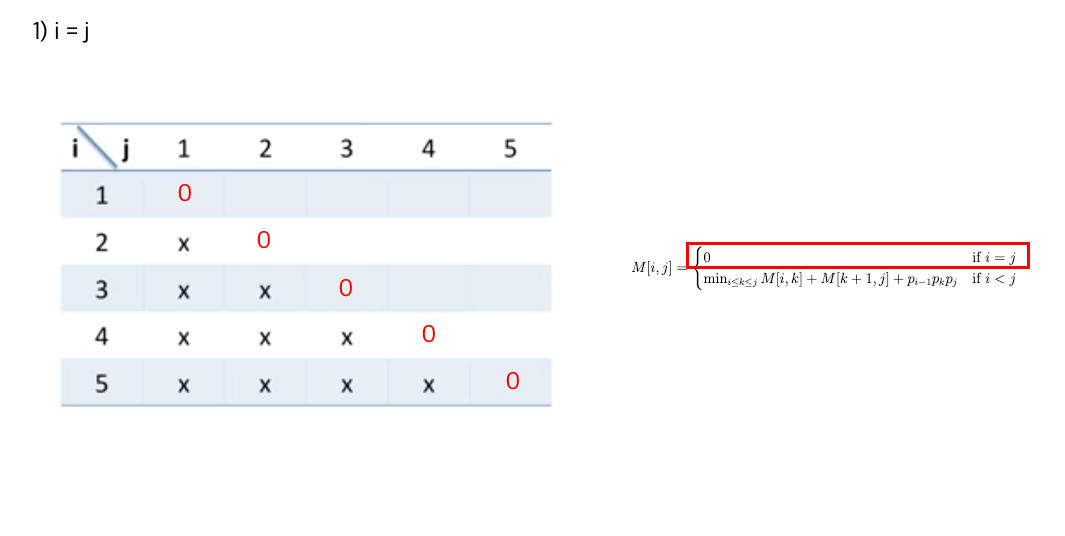
\includegraphics[width=\linewidth]{images/worksheet_3_solution_2.png}
                    \end{center}

                    \item Fill the table for $i < j$ with a spread of 1

                    \begin{center}
                    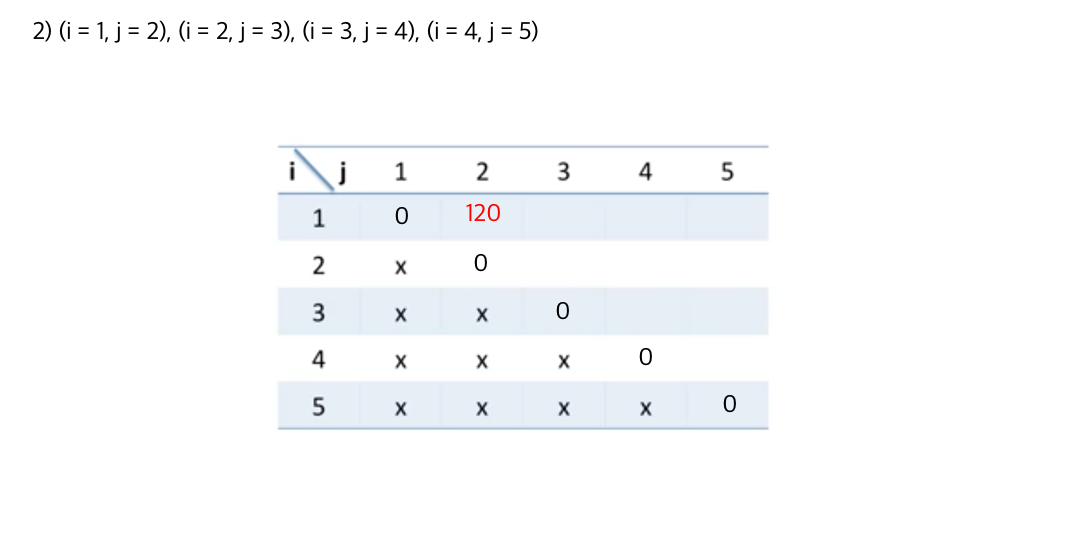
\includegraphics[width=\linewidth]{images/worksheet_3_solution_3.png}
                    \end{center}

                    since

                    \begin{itemize}
                        \item $i = 1, j = 2$

                        \begin{align}
                            M[1,2] &= \min_{1 \leq k \leq 2} (M[1,1] + M[1,2] + p_{i-1}p_kp_j)\\
                            &= \min_{1 \leq k \leq 2} (0 + 0 + p_0p_1p_2)\\
                            &= \min_{1 \leq k \leq 2} (0 + 0 + 4 \cdot 10 \cdot 3)\\
                            &= 120
                        \end{align}

                        where $p_0 = 3$ is from the dimension $3 \times 10$ of $A_1$, $p_k = 10$
                        is from the dimension of $3 \times 10$ of $A_1$.

                        \item $i = 2, j = 3$

                        \begin{align}
                            M[2,3] &= \min_{2 \leq k \leq 3} (M[2,2] + M[3,3] + p_{i-1}p_kp_j)\\
                            &= \min_{2 \leq k \leq 3} (0 + 0 + p_1p_2p_3)\\
                            &= \min_{2 \leq k \leq 3} (0 + 0 + 10 \cdot 3 \cdot 12)\\
                            &= 360
                        \end{align}

                        \item $i = 3, j = 4$

                        \begin{align}
                            M[3,4] &= \min_{3 \leq k \leq 4} (M[3,3] + M[4,4] + p_{i-1}p_kp_j)\\
                            &= \min_{3 \leq k \leq 4} (0 + 0 + p_2p_3p_4)\\
                            &= \min_{3 \leq k \leq 4} (0 + 0 + 3 \cdot 12 \cdot 20)\\
                            &= 720
                        \end{align}

                        \item $i = 4, j = 5$

                        \begin{align}
                            M[4,5] &= \min_{4 \leq k \leq 5} (M[4,4] + M[5,5] + p_{i-1}p_kp_j)\\
                            &= \min_{4 \leq k \leq 5} (0 + 0 + p_3p_4p_5)\\
                            &= \min_{4 \leq k \leq 5} (0 + 0 + 12 \cdot 20 \cdot 7)\\
                            &= 1680
                        \end{align}
                    \end{itemize}

                    \item Repeat 2 with the increased value of spread

                    \begin{center}
                    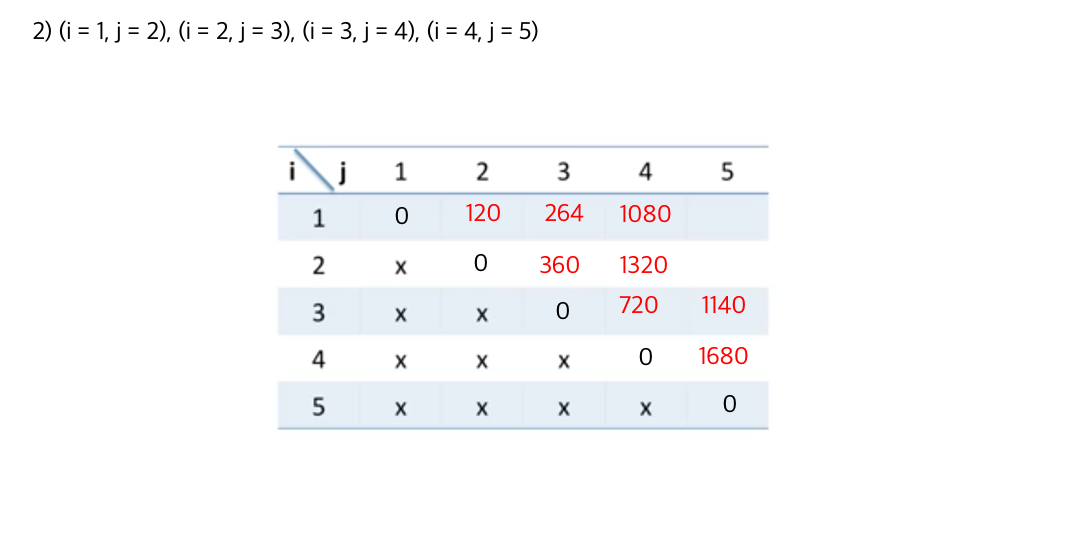
\includegraphics[width=\linewidth]{images/worksheet_3_solution_4.png}
                    \end{center}

                    \begin{itemize}
                        \item $i = 1, j = 3$

                        \bigskip

                        \underline{$k = 1$}

                        \begin{align}
                            M[1,3] &= M[1,1] + M[2,3] + p_{i-1}p_kp_j\\
                            &= 0 + 360 + p_0p_1p_3\\
                            &= 0 + 360 + 4 \cdot 10 \cdot 12\\
                            &= 0 + 360 + 480\\
                            &= 840
                        \end{align}

                        \bigskip

                        \underline{$k = 2$}

                        \begin{align}
                            M[1,3] &= M[1,2] + M[3,3] + p_{i-1}p_kp_j\\
                            &= 120 + 0 + p_0p_2p_3\\
                            &= 120 + 0 + 4 \cdot 10 \cdot 12\\
                            &= 120 + 0 + 144\\
                            &= 264
                        \end{align}

                        \bigskip

                        Thus, $\min_{1 \leq k \leq 3} M[1,3] = 264$.

                        \item $i = 2, j = 4$

                        \bigskip

                        \underline{$k = 2$}

                        \begin{align}
                            M[2,4] &= M[2,2] + M[3,4] + p_{i-1}p_kp_j\\
                            &= 0 + 720 + p_1p_2p_4\\
                            &= 0 + 720 + 10 \cdot 3 \cdot 20\\
                            &= 0 + 720 + 600\\
                            &= 1320
                        \end{align}

                        \bigskip

                        \underline{$k = 3$}

                        \begin{align}
                            M[2,4] &= M[2,2] + M[3,4] + p_{i-1}p_kp_j\\
                            &= 360 + 0 + p_1p_3p_4\\
                            &= 360 + 0 + 10 \cdot 12 \cdot 20\\
                            &= 360 + 0 + 2400\\
                            &= 2760
                        \end{align}

                        \bigskip

                        Thus, $\min_{2 \leq k \leq 4} M[2,4] = 1320$.

                        \item $i = 3, j = 5$

                        \bigskip

                        \underline{$k = 3$}

                        \begin{align}
                            M[3,5] &= M[3,3] + M[3,5] + p_{i-1}p_kp_j\\
                            &= 0 + 1680 + p_2p_3p_5\\
                            &= 0 + 1680 + 3 \cdot 12 \cdot 7\\
                            &= 0 + 1680 + 252\\
                            &= 1932
                        \end{align}

                        \bigskip

                        \underline{$k = 4$}

                        \begin{align}
                            M[3,5] &= M[3,4] + M[5,5] + p_{i-1}p_kp_j\\
                            &= 720 + 0 + p_2p_4p_5\\
                            &= 720 + 0 + 3 \cdot 20 \cdot 7\\
                            &= 720 + 420\\
                            &= 1140
                        \end{align}

                        \bigskip

                        Thus, $\min_{3 \leq k \leq 5} M[3,5] = 1140$.


                        \item $i = 2, j = 5$

                        \bigskip

                        \underline{$k = 2$}

                        \begin{align}
                            M[2,5] &= M[2,2] + M[3,5] + p_{i-1}p_kp_j\\
                            &= 0 + 1140 + p_1p_2p_5\\
                            &= 0 + 1140 + 10 \cdot 3 \cdot 7\\
                            &= 0 + 1140 + 210\\
                            &= 1350
                        \end{align}

                        \bigskip

                        \underline{$k = 3$}

                        \begin{align}
                            M[2,5] &= M[2,3] + M[4,5] + p_{i-1}p_kp_j\\
                            &= 360 + 1680 + p_1p_3p_5\\
                            &= 2040 + 10 \cdot 12 \cdot 7\\
                            &= 2040 + 840\\
                            &= 2880
                        \end{align}

                        \bigskip

                        \underline{$k = 4$}

                        \begin{align}
                            M[2,5] &= M[2,4] + M[5,5] + p_{i-1}p_kp_j\\
                            &= 1320 + p_1p_3p_5\\
                            &= 1320 + 10 \cdot 20 \cdot 7\\
                            &= 1320 + 1400\\
                            &= 2720
                        \end{align}

                        \bigskip

                        Thus, $\min_{2 \leq k \leq 5} M[2,5] = 1350$.

                        \item $i = 1, j = 5$

                        \bigskip

                        \underline{$k = 1$}

                        \begin{align}
                            M[1,5] &= M[1,1] + M[3,5] + p_{i-1}p_kp_j\\
                            &= 0 + 1350 + p_0p_1p_5\\
                            &= 0 + 1350 + 4 \cdot 10 \cdot 7\\
                            &= 0 + 1350 + 280\\
                            &= 1630
                        \end{align}

                        \bigskip

                        \underline{$k = 2$}

                        \begin{align}
                            M[1,5] &= M[1,2] + M[3,5] + p_{i-1}p_kp_j\\
                            &= 120 + 1140 + p_0p_2p_5\\
                            &= 120 + 1140 + 4 \cdot 3 \cdot 7\\
                            &= 1260 + 84\\
                            &= 1344
                        \end{align}

                        \bigskip

                        \underline{$k = 3$}

                        \begin{align}
                            M[1,5] &= M[1,3] + M[4,5] + p_{i-1}p_kp_j\\
                            &= 264 + 1680 + p_0p_3p_5\\
                            &= 264 + 1680 + 4 \cdot 12 \cdot 7\\
                            &= 1944 + 336\\
                            &= 2280
                        \end{align}

                        \bigskip

                        \underline{$k = 4$}

                        \begin{align}
                            M[1,5] &= M[1,4] + M[5,5] + p_{i-1}p_kp_j\\
                            &= 1080 + 0 + p_0p_4p_5\\
                            &= 1080 + 4 \cdot 20 \cdot 7\\
                            &= 1080 + 560\\
                            &= 1640
                        \end{align}

                        \bigskip

                        Thus, $\min_{1 \leq k \leq 5} M[1,5] = 1344$.

                    \end{itemize}


                \end{enumerate}

                \item \textbf{Constructing the Optimal Solution (Needs revision)}

                \bigskip

                \begin{center}
                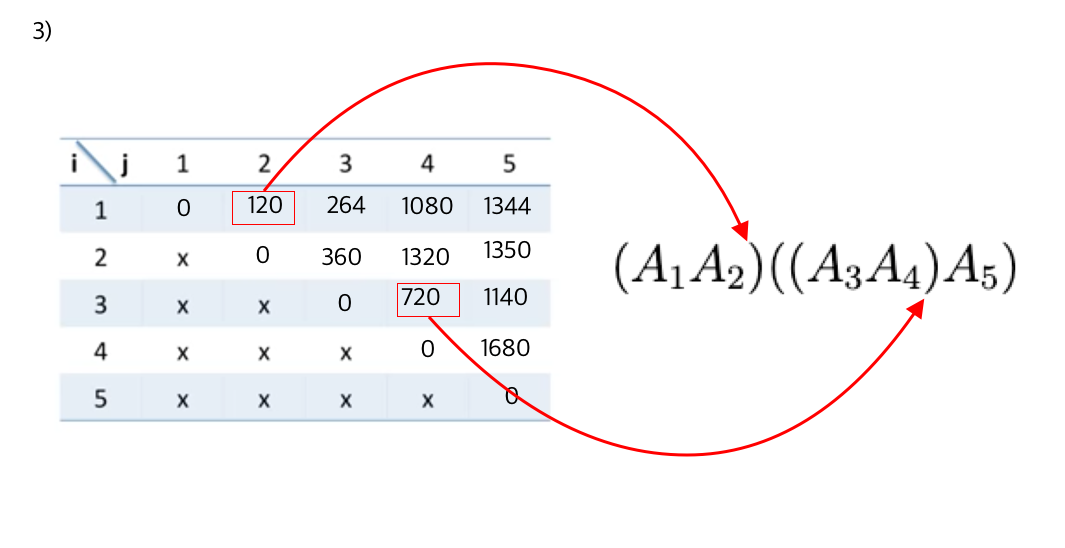
\includegraphics[width=\linewidth]{images/worksheet_3_solution_5.png}
                \end{center}

                \bigskip

                So, the optimal solution is $(A_1 A_2)((A_3A_4)A_5)$

            \end{enumerate}
        \end{itemize}

        \bigskip

        \underline{\textbf{References:}}

        \bigskip

        \begin{enumerate}[1)]
            \item CSBreakdown, Chain Multiplication - Dynamic Programming, \href{https://www.youtube.com/watch?v=GMzVeWpyTN0}{link}
            \item University of Maryland, CMSC351 - Fall 2014 Homework \# 4, \href{https://www.cs.umd.edu/class/fall2014/cmsc351/HW/hw4-solutions.pdf}{link}
        \end{enumerate}
    \end{itemize}

    \item

    \bigskip

    \begin{lstlisting}
    procedure MATRIX-CHAIN-MULTIPLY(A,s,i,j)
        if i == j then
            return A[i]
        end if

        if i < j
            a = MATRIX-CHAIN-MULTIPLY(A,s,i,s[i,j])
            b = MATRIX-CHAIN-MULTIPLY(A,s,s[i,j] + 1,j)

            return MATRIX-CHAIN-MULTIPLY(a,b)

        end if

    end procedure
    \end{lstlisting}

    \bigskip

    \underline{\textbf{Example:}}

    \bigskip

    \begin{itemize}
        \item \textit{MATRIX-CHAIN-ORDER} computes the table $s$ containing optimal costs
        \item $s$ table consists of $k$ value at which $m[i,j]$ is minimum!!

        \bigskip

        $A_{1..s[1,n]}A_{s[1,n]+1..n}$

        \bigskip

        \item Table of optimal costs $m$ is used with table $s$ to construct solution to
        matrix-chain multiplication problem

    \end{itemize}

    \item
    \setcounter{equation}{0}
    \bigskip

    First, we need to determine the total number of times $m[i,j]$ is referred in the
    innermost loop.

    \bigskip

    We know from the header that the loop runs from $k = i$ to $k = j - 1$.

    \bigskip

    Using this fact, we can write the innermost loop has $j - i = l - 1$ iterations.

    \bigskip

    Since $m[i.j]$ is referred twice, the total number of $m[i,j]$ referred
    in the loop is:

    \begin{align}
        (l - 1)2
    \end{align}

    \bigskip

    Second, we need to determine the total number of times $m[i,j]$ is referred in the
    intermediate loop

    \bigskip

    We know from the header that the loop runs from $i = 1$ to $i = n - l + 1$.

    \bigskip

    Using this fact, we can write the intermediate loop runs $n - l + 1$ iterations.

    \bigskip

    Since each iteration referrs $m[i,j]$ $(l - 1)2$ many times, the total number
    of times $m[i,j]$ is referred in the itnermediate loop is:

    \bigskip

    \begin{align}
        (n - l + 1)(l - 1)2
    \end{align}

    \bigskip

    Finally, we need to determine the total number of times $m[i,j]$ is referenced
    in the outermost loop.

    \bigskip

    We know from the header that the loop runs from $l = 2$ to $n$.

    \bigskip

    Since each iteration referrs $m[i,j]$ $(n - l + 1)(l - 1)2$ many times, the total number
    of times $m[i,j]$ is referred in the outermost loop is:

    \bigskip

    \begin{align}
        \sum\limits_{l=2}^{n} (n - l + 1)(l - 1)2 &= 2\sum\limits_{l'=1}^{n-1} (n - l')(l')\\
        &= 2 \Bigl[\sum\limits_{l'=1}^{n-1} nl' - (l')^2 \Bigr]\\
        &= 2 \Bigl[ n \sum\limits_{l'=1}^{n-1} l' - \sum\limits_{l'=1}^{n-1} (l')^2 \Bigr]\\
        &= 2 \Bigl[ n \sum\limits_{l'=1}^{n-1} l' - \sum\limits_{l'=1}^{n-1} (l')^2 \Bigr]\\
        &= 2 \Bigl[ n \sum\limits_{l'=0}^{n-1} l' - \sum\limits_{l'=0}^{n-1} (l')^2 \Bigr]\\
        &= 2 \Bigl[ \frac{(n-1)n^2}{2} - \frac{(n-1)n(2n-1)}{6} \Bigr]\\
        &= 2 \Bigl[ \frac{n^3 - n^2}{2} - \frac{(n-1)n(2n-1)}{6} \Bigr]\\
        &= 2 \Bigl[ \frac{n^3 - n^2}{2} - \frac{(n^2-n)(2n-1)}{6} \Bigr]\\
        &= 2 \Bigl[ \frac{n^3 - n^2}{2} - \frac{(3n^3-3n^2 + n)}{6} \Bigr]\\
        &= 2 \Bigl[ \frac{3n^3 - 3n^2}{6} - \frac{(3n^3-3n^2 + n)}{6} \Bigr]\\
        &= 2 \Bigl[ \frac{n^3 - n}{6}\Bigr]\\
        &= \frac{n^3 - n}{3}
    \end{align}



    % \bigskip

    % \underline{\textbf{Rough Work:}}
    % \setcounter{equation}{0}
    % \bigskip

    % \begin{enumerate}[1.]
    %     \item Find equation that determines the total number of times $m[i,j]$ is referenced

    %     \begin{itemize}
    %         \item Determine the total number of times $m[i,j]$ is referenced in the
    %         innermost loop

    %         \bigskip

    %         First, we need to determine the total number of times $m[i,j]$ is referred in the
    %         innermost loop.

    %         \begin{mdframed}
    %         We know from the header that the loop runs from $k = i$ to $k = j - 1$.

    %         \bigskip

    %         Using this fact, we can write the innermost loop has $j - i = l - 1$ iterations.

    %         \bigskip

    %         Since $m[i.j]$ is referred twice, the total number of $m[i,j]$ referred
    %         in the loop is:

    %         \begin{align}
    %             (l - 1)2
    %         \end{align}

    %         \end{mdframed}

    %         \item Determine the total number of times $m[i,j]$ is referenced in the
    %         intermediate loop

    %         \bigskip

    %         Second, we need to determine the total number of times $m[i,j]$ is referred in the
    %         intermediate loop

    %         \begin{mdframed}
    %         We know from the header that the loop runs from $i = 1$ to $i = n - l + 1$.

    %         \bigskip

    %         Using this fact, we can write the intermediate loop runs $n - l + 1$ iterations.

    %         \bigskip

    %         Since each iteration referrs $m[i,j]$ $(l - 1)2$ many times, the total number
    %         of times $m[i,j]$ is referred in the itnermediate loop is:

    %         \bigskip

    %         \begin{align}
    %             (n - l + 1)(l - 1)2
    %         \end{align}

    %         \end{mdframed}

    %         \item Determine the total number of times $m[i,j]$ is referenced in the
    %         outermost loop

    %         \bigskip

    %         Finally, we need to determine the total number of times $m[i,j]$ is referenced
    %         in the outermost loop.

    %         \bigskip

    %         \begin{mdframed}
    %         We know from the header that the loop runs from $l = 2$ to $n$.

    %         \bigskip

    %         Since each iteration referrs $m[i,j]$ $(n - l + 1)(l - 1)2$ many times, the total number
    %         of times $m[i,j]$ is referred in the outermost loop is:

    %         \bigskip

    %         \begin{align}
    %             \sum\limits_{l=2}^{n} (n - l + 1)(l - 1)2 &= 2\sum\limits_{l'=1}^{n-1} (n - l')(l')\\
    %             &= 2 \Bigl[\sum\limits_{l'=1}^{n-1} nl' - (l')^2 \Bigr]\\
    %             &= 2 \Bigl[ n \sum\limits_{l'=1}^{n-1} l' - \sum\limits_{l'=1}^{n-1} (l')^2 \Bigr]\\
    %             &= 2 \Bigl[ n \sum\limits_{l'=1}^{n-1} l' - \sum\limits_{l'=1}^{n-1} (l')^2 \Bigr]\\
    %             &= 2 \Bigl[ n \sum\limits_{l'=0}^{n-1} l' - \sum\limits_{l'=0}^{n-1} (l')^2 \Bigr]\\
    %             &= 2 \Bigl[ \frac{(n-1)n^2}{2} - \frac{(n-1)n(2n-1)}{6} \Bigr]\\
    %             &= 2 \Bigl[ \frac{n^3 - n^2}{2} - \frac{(n-1)n(2n-1)}{6} \Bigr]\\
    %             &= 2 \Bigl[ \frac{n^3 - n^2}{2} - \frac{(n^2-n)(2n-1)}{6} \Bigr]\\
    %             &= 2 \Bigl[ \frac{n^3 - n^2}{2} - \frac{(3n^3-3n^2 + n)}{6} \Bigr]\\
    %             &= 2 \Bigl[ \frac{3n^3 - 3n^2}{6} - \frac{(3n^3-3n^2 + n)}{6} \Bigr]\\
    %             &= 2 \Bigl[ \frac{n^3 - n}{6}\Bigr]\\
    %             &= \frac{n^3 - n}{3}
    %         \end{align}

    %         \end{mdframed}
    %     \end{itemize}

    % \end{enumerate}

    \bigskip

    \underline{\textbf{Notes:}}

    \bigskip

    \begin{itemize}
        \item Hint from equation $A.3$

        \bigskip

        $\sum\limits_{k=0}^n k^2 = \frac{n(n+1)(2n+1)}{6}$

        \item I feel the need to gain more insight regarding the question's `other table
        entries in a call of MATRIX-CHAIN-ORDER'. What does `other table entries' mean?

        \bigskip

        \underline{\textbf{Answer:}}

        \begin{center}
        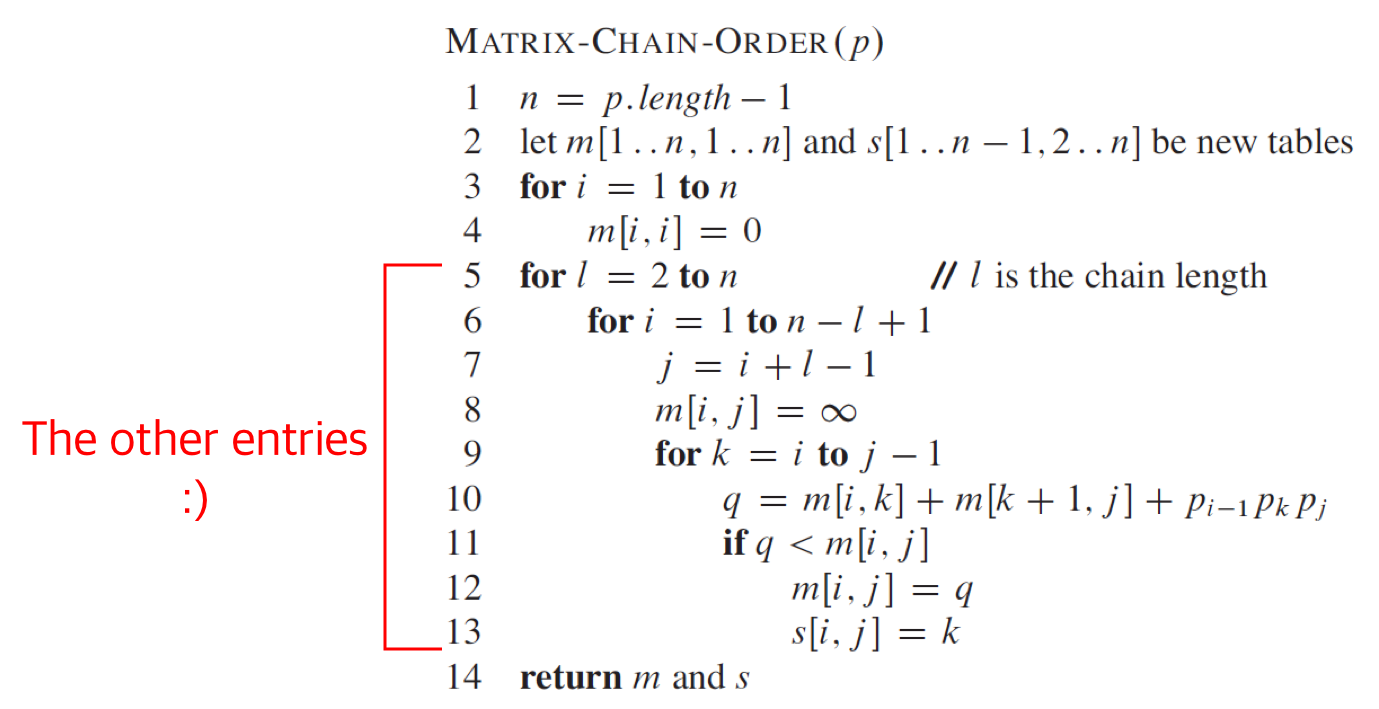
\includegraphics[width=\linewidth]{images/worksheet_3_solution_6.png}
        \end{center}

        \item In the problem `$m[i,j]$ is referenced' refers to $m[i,j]$ used in assignments $q = m[i,j] ...$

        \begin{center}
        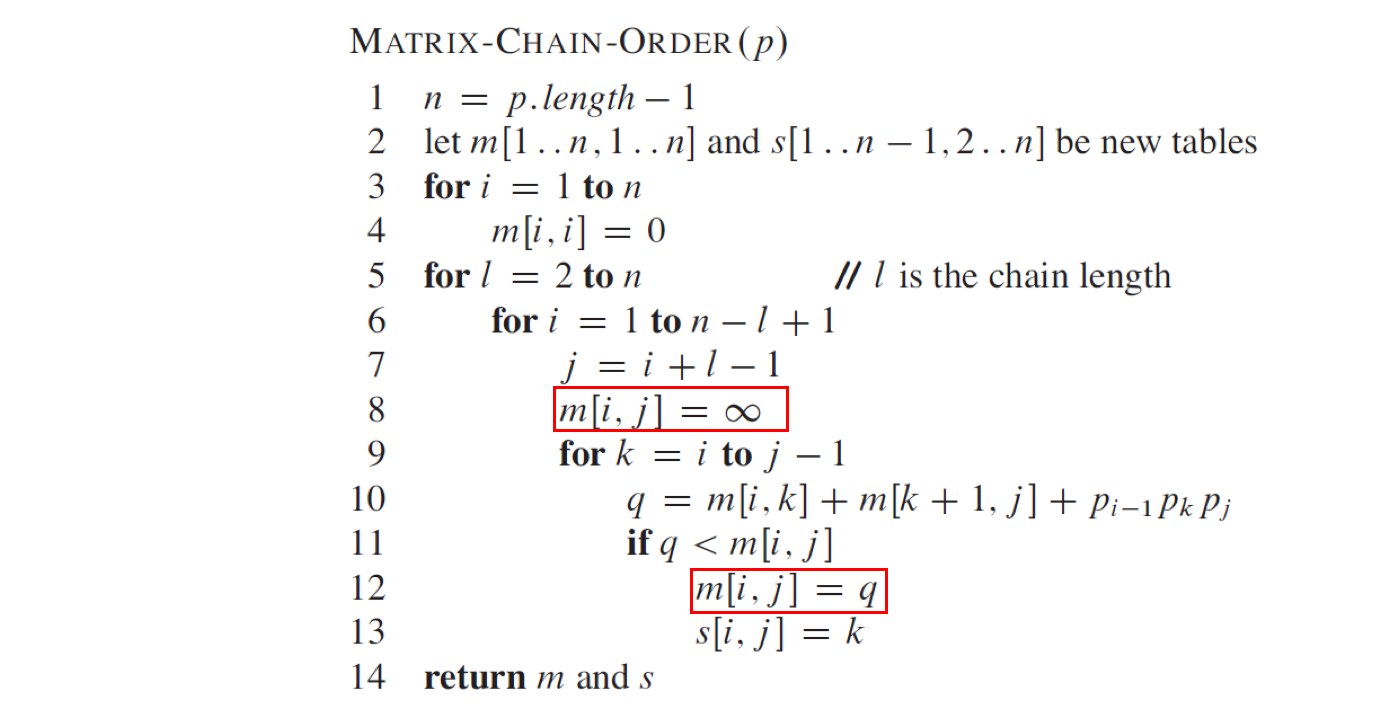
\includegraphics[width=\linewidth]{images/worksheet_3_solution_7.png}
        \end{center}
    \end{itemize}

    \item

    \underline{\textbf{Solution}}

    \bigskip

    \begin{center}
    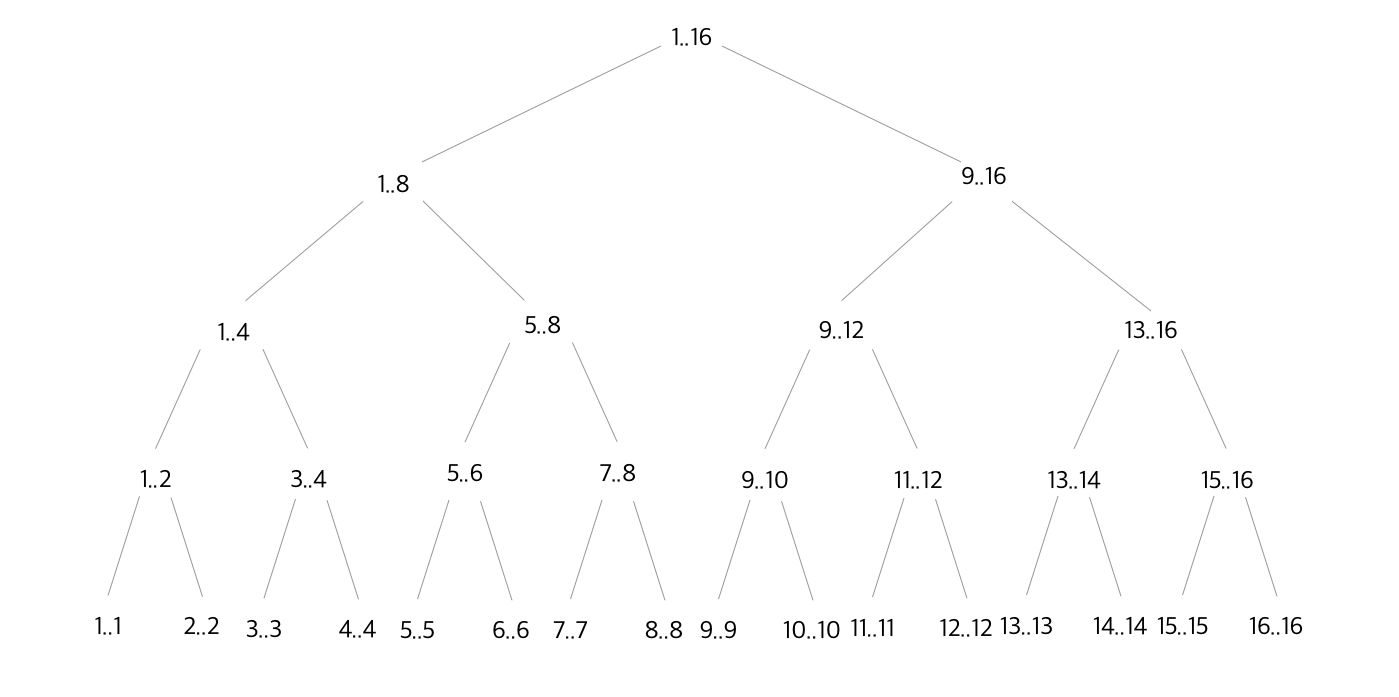
\includegraphics[width=\linewidth]{images/worksheet_3_solution_11.png}
    \end{center}

    Memoization fails to speed up the algorithm because it lacks overlapping subproblems.

    \bigskip

    \underline{\textbf{Notes:}}

    \bigskip

    \begin{itemize}
        \item Elements of Dynamic Programming
        \begin{itemize}
            \item Optimal Substructure
            \begin{itemize}
                \item Is the first step to solving dynamic programming problem
                \item Exists if an optimal solution to the problem contains within it optimal
                solution to subproblems
            \end{itemize}
            \item Overlapping Subproblems

            \begin{itemize}
                \item Is the second step to solving dynamic programming
                \item Exists when an algorithm revisits the same problem repeatedly
            \end{itemize}
            \item Memoization
            \begin{itemize}
                \item Maintains an entry in a table for the solution to each subproblem
                \item Ensures that a method doesn't run for the same inputs more than once
            \end{itemize}
        \end{itemize}

        \item Top-Down Dynamic Programming
        \begin{itemize}
            \item Uses recursion
            \item Is preferred
            \begin{itemize}
                \item When all sub-solutions need to be solved
                \item Because it's easier
            \end{itemize}
        \end{itemize}


        \begin{center}
        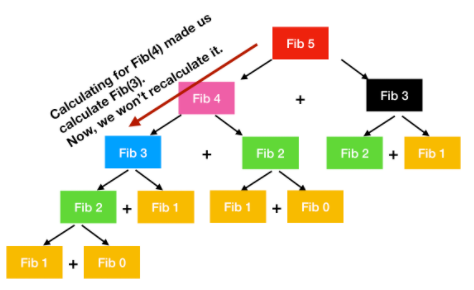
\includegraphics[width=0.7\linewidth]{images/worksheet_3_solution_8.png}
        \end{center}

        \item Bottom-Up Dynamic Programming
        \begin{itemize}
            \item Uses for-loop
            \item Is preferred
            \begin{itemize}
                \item When all sub-solutions need to be solved
                \item Because it is sometimes faster (No recursive call and no unnecessary Random Memory access)
            \end{itemize}
            \item Is preferred when not all sub-solutions need to be computed
        \end{itemize}

        \begin{center}
        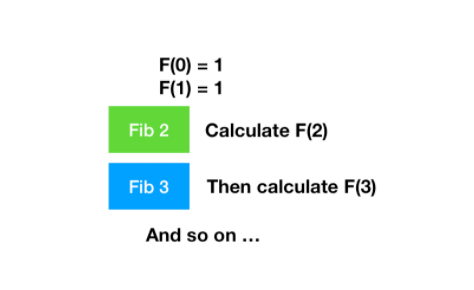
\includegraphics[width=0.7\linewidth]{images/worksheet_3_solution_9.png}
        \end{center}

        \item Merge Sort

        \begin{itemize}
            \item How it works

            \begin{enumerate}[1.]
                \item Find the middle point to divide the array into two halves
                \item Call mergeSort for first half
                \item Call mergeSort for second half
                \item Merge two halves in sorted order
            \end{enumerate}
        \end{itemize}

        \begin{center}
        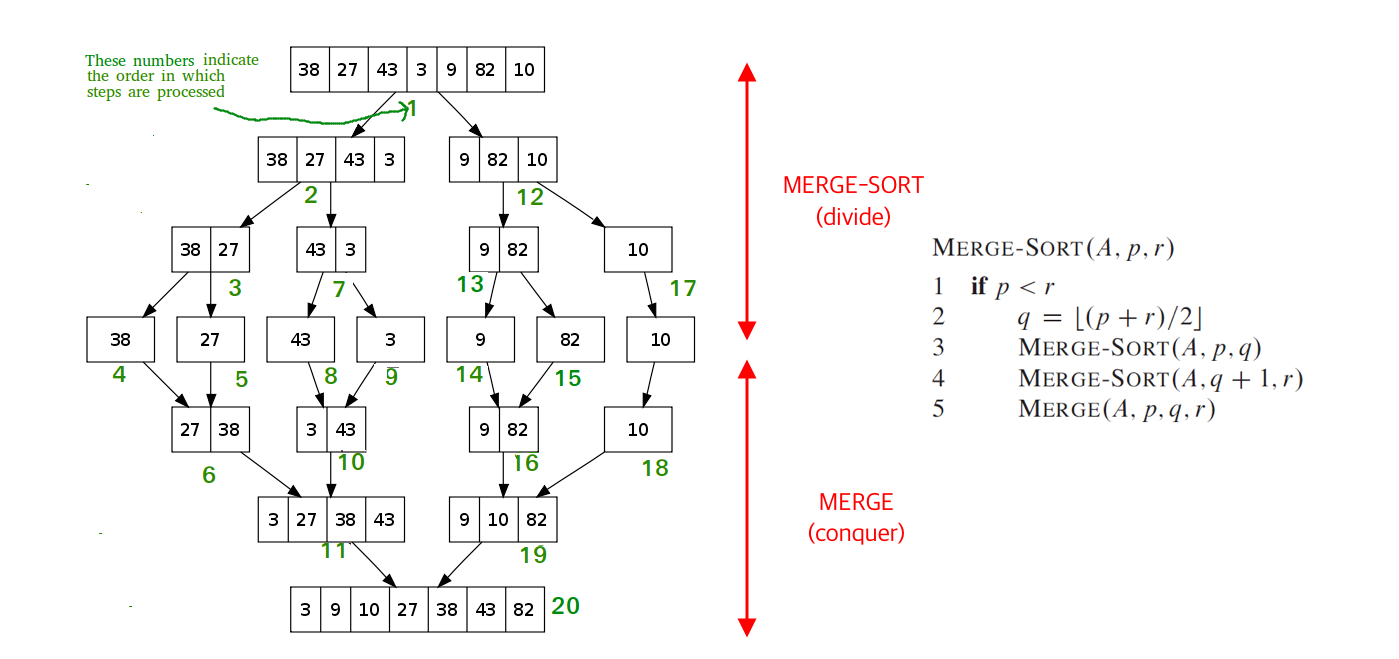
\includegraphics[width=\linewidth]{images/worksheet_3_solution_10.png}
        \end{center}

        \bigskip

        \underline{\textbf{References}}

        \bigskip

        \begin{enumerate}[1)]
            \item
        \end{enumerate}

    \end{itemize}

    \item

    Yes. This problem does exhibit optimal substructure

    \begin{proof}
        Assume that the optimal structure of $A_iA_{i+1}..A_j$ exists. That is,
        there exists some $k \in \mathbb{N} - \{0\}$ such that the following parenthesis $(A_{i..k})(A_{k+1..j})$
        produces maximum operation cost.

        \bigskip

        I need to show that the substructures $A_{i..k}$ and $A_{k+1..j}$ are also optimal.

        \bigskip

        I will do so in parts.

        \bigskip

        \underline{\textbf{Part 1 (Proving optimal substructure of $A_{i..k}$)}}

        \bigskip

        Assume for the sake of contradiction that the substructure $A_{i..k}$ is
        not optimal.

        \bigskip

        Then, we can write that there exists some $k' \in \mathbb{N} - \{0\}$ such that
        $(A_{i...k'})(A_{k'+1..k})$ has larger operation cost than $(A_{i..k})$.

        \bigskip

        Then, we can write that $((A_{i...k'})(A_{k'+1..k}))(A_{k+1..j})$ has larger
        operation costs than $(A_{i..k})(A_{k+1..j})$, which contradicts the original assumption that
        $(A_{i..k})(A_{k+1..j})$ has maximum operation cost.

        \bigskip

        Thus, $(A_{i..k})$ must be optimal.


        \bigskip

        \underline{\textbf{Part 2 (Proving optimal substructure of $A_{k+1..j}$)}}

        \bigskip

        This proof is nearly verbatim as part 1, where the only difference is using $A_{k+1..j}$
        instead of $A_{i..j}$.
    \end{proof}

    \bigskip

    \underline{\textbf{Notes:}}

    \bigskip

    \begin{itemize}
        \item A problem has \textbf{optimal substructure} if an optimal solution
        can be constructed from optimal solutions of its subproblems. $^{[3]}$

        \item Showing optimal subtructure for the original Matrix-Chain Multiplication problem

        \bigskip

        \begin{mdframed}
        Assume that the optimal structure of $A_iA_{i+1}..A_j$ exists. That is,
        there exists some $k \in \mathbb{N} - \{0\}$ such that the following parenthesis $(A_{i..k})(A_{k+1..j})$
        produces minimum operation cost.

        \bigskip

        I need to show that the substructures $A_{i..k}$ and $A_{k+1..j}$ are also optimal.

        \bigskip

        I will do so in parts.

        \bigskip

        \underline{\textbf{Part 1 (Proving optimal substructure of $A_{i..k}$)}}

        \bigskip

        Assume for the sake of contradiction that the substructure $A_{i..k}$ is
        not optimal.

        \bigskip

        Then, we can write that there exists some $k' \in \mathbb{N} - \{0\}$ such that
        $(A_{i...k'})(A_{k'+1..k})$ has smaller operation cost than $(A_{i..k})$.

        \bigskip

        Then, we can write that $((A_{i...k'})(A_{k'+1..k}))(A_{k+1..j})$ has smaller
        operation costs than $(A_{i..k})(A_{k+1..j})$, which contradicts the original assumption that
        $(A_{i..k})(A_{k+1..j})$ has minimum operation cost.

        \bigskip

        Thus, $(A_{i..k})$ must be optimal.


        \bigskip

        \underline{\textbf{Part 2 (Proving optimal substructure of $A_{k+1..j}$)}}

        \bigskip

        This proof is nearly verbatim as part 1, where the only difference is using $A_{k+1..j}$
        instead of $A_{i..j}$.

        \end{mdframed}
    \end{itemize}

    \bigskip

    \underline{\textbf{References:}}

    \bigskip

    \begin{enumerate}[1)]
        \item CSBreakdown, Chain Multiplication - Dynamic Programming, \href{https://www.youtube.com/watch?v=GMzVeWpyTN0}{link}
        \item CodeScope, Dynamic Programming, \href{https://www.codesdope.com/course/algorithms-dynamic-programming/}{link}
        \item Wikipedia, Optimal Substructure, \href{https://en.wikipedia.org/wiki/Optimal_substructure}{link}
    \end{enumerate}

    \item

        Let $<2,10,20,5>$.

        \bigskip

        Then, we see that $p_0p_1p_3$ is minimum, and by  Professor Capulet's claim,
        splitting at $k = 1$ should result in minimum-cost matrix multiplication.

        \bigskip

        But we have

        \begin{center}
            \begin{tabular}{|c|c|c|c|}
                \hline
                m & 1 & 2 & 3\\
                \hline
                1 & 0 & 400 & 600\\
                \hline
                2 & x & 0 & 1000\\
                \hline
                3 & x & x & 0\\
                \hline
            \end{tabular}

            \begin{tabular}{|c|c|c|c|}
                \hline
                s & 1 & 2 & 3\\
                \hline
                1 & 0 & 1 & \color{red}2\color{black}\\
                \hline
                2 & x & 0 & 2\\
                \hline
                3 & x & x & 0\\
                \hline
            \end{tabular}
        \end{center}

        \bigskip

        And the minimum-cost matrix multiplication occurs when $A_{i..j}$ is splitted
        at $k = 2$.

        \bigskip

        Thus, Professor Capulet's claim is false.

    % \bigskip

    % \underline{\textbf{Rough Work:}}

    % \bigskip

    % \begin{itemize}
    %     \item $<8,10,20,5>$ $\to$ Meets Professor Capulet's Claim \& Not solution

    %     \bigskip

    %     We see that $p_0p_1p_3$ is minimum. So, by  Professor Capulet's claim, splitting
    %     at $k = 1$ should result in minimum-cost matrix multiplication.

    %     \bigskip

    %     And we have

    %     \begin{center}
    %         \begin{tabular}{|c|c|c|c|}
    %             \hline
    %             m & 1 & 2 & 3\\
    %             \hline
    %             1 & 0 & 1600 & 1400\\
    %             \hline
    %             2 & x & 0 & 1000\\
    %             \hline
    %             3 & x & x & 0\\
    %             \hline
    %         \end{tabular}

    %         \begin{tabular}{|c|c|c|c|}
    %             \hline
    %             s & 1 & 2 & 3\\
    %             \hline
    %             1 & 0 & 1 & \color{red}1\color{black}\\
    %             \hline
    %             2 & x & 0 & 2\\
    %             \hline
    %             3 & x & x & 0\\
    %             \hline
    %         \end{tabular}
    %     \end{center}

    %     \item $<8,10,2,5>$ $\to$ Meets Professor Capulet's Claim \& Not solution

    %     \bigskip

    %     We see that $p_0p_2p_3$ is minimum. So, by  Professor Capulet's claim, splitting
    %     at $k = 2$ should result in minimum-cost matrix multiplication.

    %     \bigskip

    %     And we have

    %     \begin{center}
    %         \begin{tabular}{|c|c|c|c|}
    %             \hline
    %             m & 1 & 2 & 3\\
    %             \hline
    %             1 & 0 & 160 & 260\\
    %             \hline
    %             2 & x & 0 & 100\\
    %             \hline
    %             3 & x & x & 0\\
    %             \hline
    %         \end{tabular}

    %         \begin{tabular}{|c|c|c|c|}
    %             \hline
    %             s & 1 & 2 & 3\\
    %             \hline
    %             1 & 0 & 1 & \color{red}2\color{black}\\
    %             \hline
    %             2 & x & 0 & 2\\
    %             \hline
    %             3 & x & x & 0\\
    %             \hline
    %         \end{tabular}
    %     \end{center}

    %     \item $<2,10,20,5>$ $\to$ Solution

    %     \bigskip

    %     We see that $p_0p_1p_3$ is minimum. So, by  Professor Capulet's claim, splitting
    %     at $k = 1$ should result in minimum-cost matrix multiplication.

    %     \bigskip

    %     But we have

    %     \begin{center}
    %         \begin{tabular}{|c|c|c|c|}
    %             \hline
    %             m & 1 & 2 & 3\\
    %             \hline
    %             1 & 0 & 400 & 600\\
    %             \hline
    %             2 & x & 0 & 1000\\
    %             \hline
    %             3 & x & x & 0\\
    %             \hline
    %         \end{tabular}

    %         \begin{tabular}{|c|c|c|c|}
    %             \hline
    %             s & 1 & 2 & 3\\
    %             \hline
    %             1 & 0 & 1 & \color{red}2\color{black}\\
    %             \hline
    %             2 & x & 0 & 2\\
    %             \hline
    %             3 & x & x & 0\\
    %             \hline
    %         \end{tabular}
    %     \end{center}

    %     \bigskip

    %     So, professor Capulet's claim is false
    % \end{itemize}

    \bigskip

    \underline{\textbf{Notes:}}

    \bigskip

    \begin{itemize}
        \item I need to find the matrices $A_i, ..., A_j$ where the total operating cost of Professor Capulet's
        method is bigger than the properly parenthesized solution
        \item I feel the need for clarafication regarding the phrase `always choosing the matrix $A_k$ at which to split the product...'
        Is $k$ in $A_k$ the same in any matrix multiplications $A_iA_{i+1}...A_j$?

        \bigskip

        \underline{\textbf{Answer:}}

        \bigskip

        No. $k$ in $A_k$ is the value that makes $p_{i-1}p_kp_j$ minimum.
    \end{itemize}

    \item

    \bigskip

    \underline{\textbf{Solution:}}

    \bigskip

    \begin{center}
    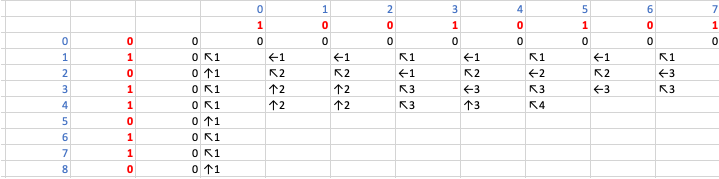
\includegraphics[width=\linewidth]{images/worksheet_3_solution_20.png}
    \end{center}

    \bigskip

    So, the LCS of $<1,0,0,1,0,1,0,1>$ and $<0,1,0,1,1,0,1,1,0>$ is `101101'.

    \bigskip

    \underline{\textbf{Notes:}}

    \bigskip

    \begin{itemize}
        \item Longest Common Sequence
        \begin{itemize}
            \item Goal is to find the longest common subsequence in $X = <x_1, x_2, ..., x_n>$ and $Y = <y_1, y_2, ... , y_n>$
            \item e.g. Given two substrings $s_1 = <M,U,N,G>$ and $s_2 = <U,N,I,V,E,R,S,I,T,Y>$, the longest
            substring is `$<U,N>$'.
            \item Steps
            \begin{enumerate}[1.]
                \item Verify Optimal Substructure
                \item Create Recursive Solution

                \bigskip

                \begin{align}
                    M[i,j] = \begin{cases}
                        0 & \text{$i = 0$, or $j = 0$}\\
                        c[i-1,j-1]+1 & \text{if $i,j > 0$ and $a_i = b_j$}\\
                        Max(C_{i,j-1},C_{i-1,j}) & \text{if $i,j > 0$ $a_i \neq b_j$}
                    \end{cases}
                \end{align}

                \item Computing the length of an LCS

                \bigskip

                \begin{itemize}
                    \item Top-Down Solution
                    \item Bottom-Top Solution

    \begin{lstlisting}[mathescape=true]
    LCS-LENGTH(X,Y)
        m = X.length
        n = Y.length

        let b[1..m, 1..n] and c[0..m, 0..n] be new tables

        for i = 1 to m
            c[i,0] = 0

        for j = 0 to n
            c[0,j] = 0

        for i = 1 to m
            for j = 1 to n
                if x[i] == y[i]
                    c[i,j] = c[i-1,j-1] + 1
                    b[i,j] = '$\nwarrow$'

                elseif c[i-1, j] $\geq$ c[i,j-1]
                    c[i,j] = c[i,j-1]
                    b[i,j] = '$\uparrow$'

                else
                    c[i,j] = c[i,j-1]
                    b[i,j] = '$\leftarrow$'

        return c and b
    \end{lstlisting}
                \end{itemize}
                \item Constructing an LCS

                \bigskip

                \underline{\textbf{Steps:}}

                \bigskip

                \begin{enumerate}[1)]
                    \item Fill $i = 0$ or $j = 0$ with 0

                    \begin{center}
                    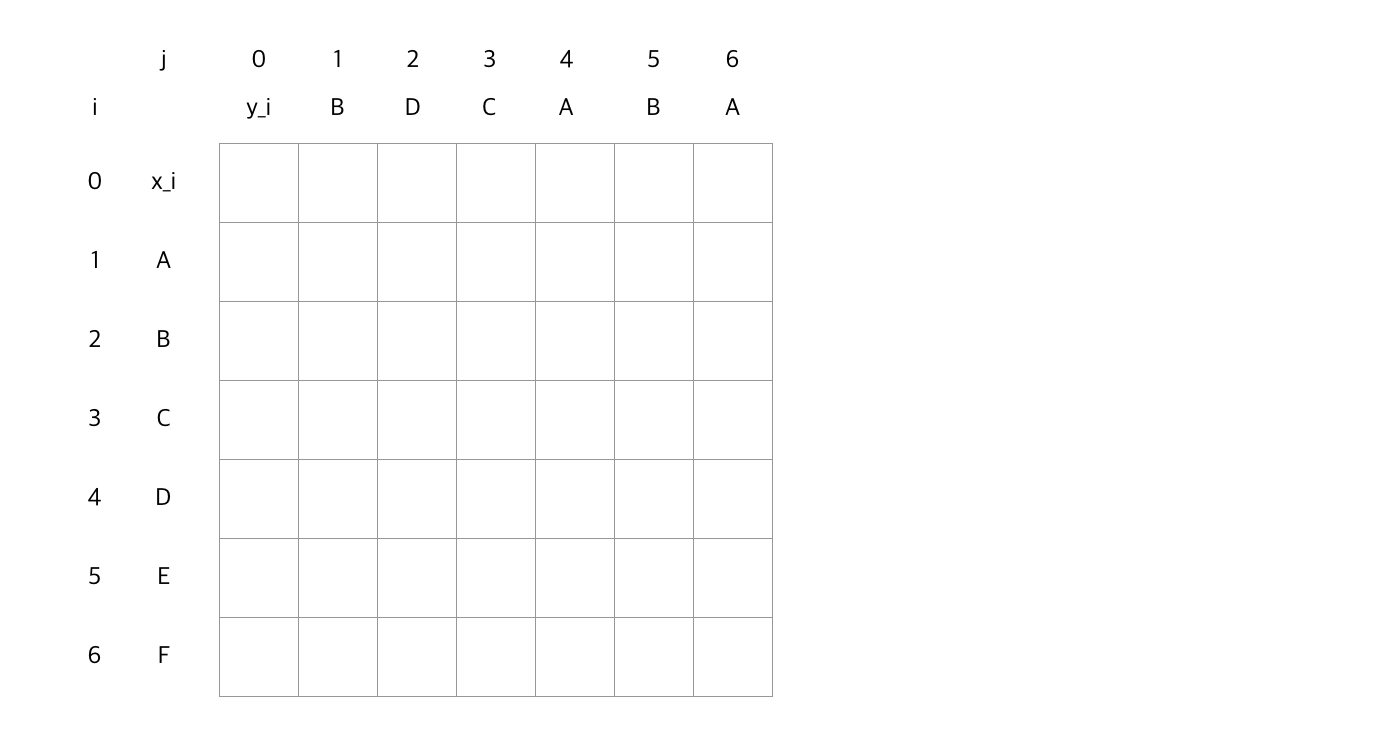
\includegraphics[width=\linewidth]{images/worksheet_3_solution_12.png}
                    \end{center}

                    \item Compute $i = 1$ (needs revision)

                    \bigskip

                    \begin{center}
                    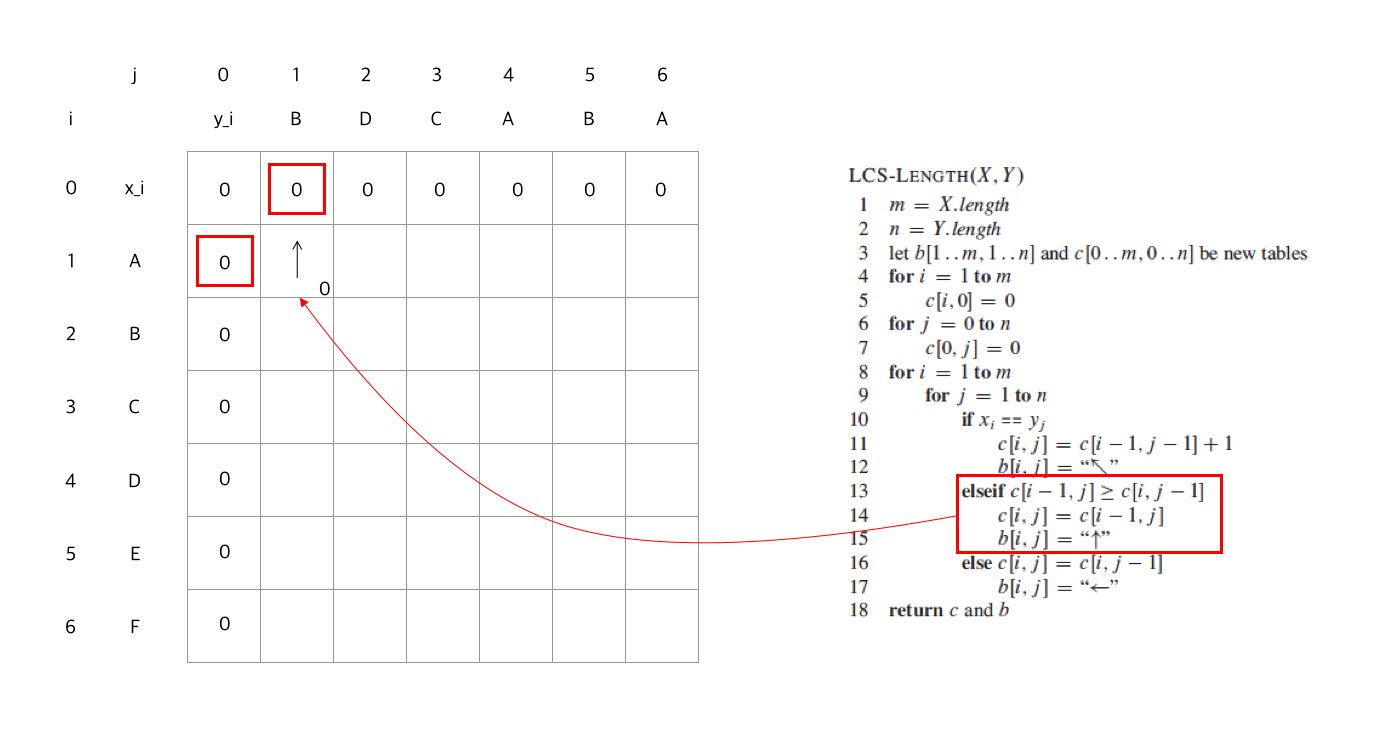
\includegraphics[width=\linewidth]{images/worksheet_3_solution_13.png}
                    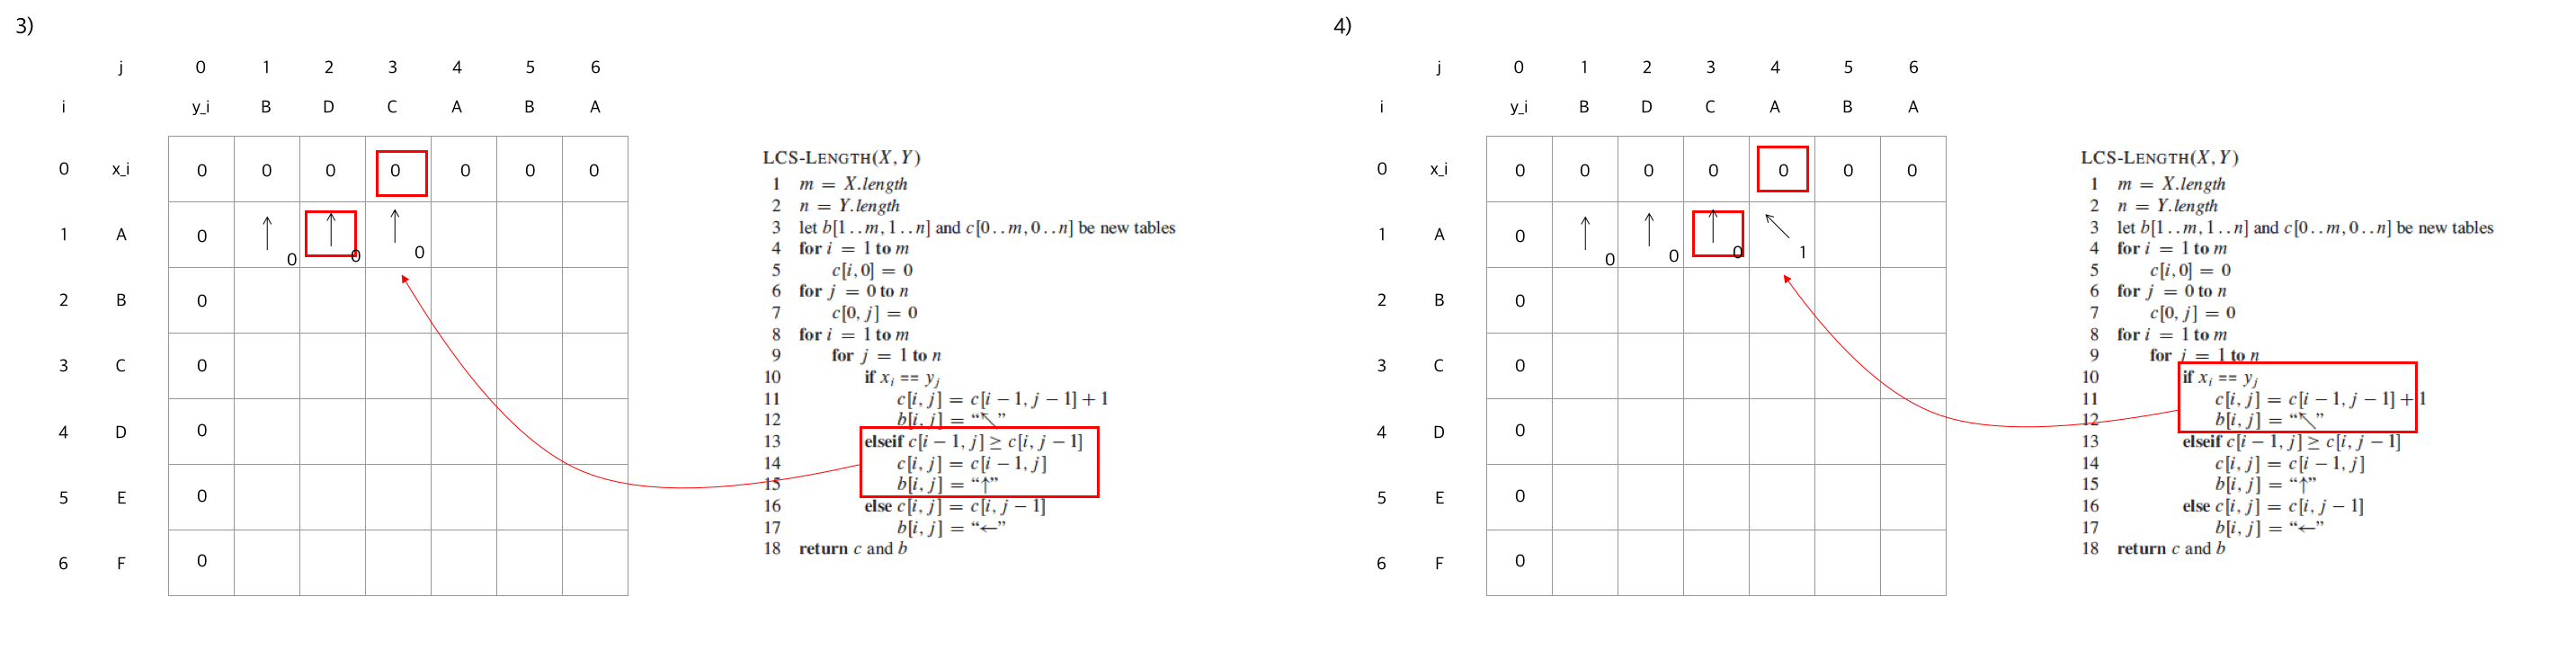
\includegraphics[width=\linewidth]{images/worksheet_3_solution_14.png}
                    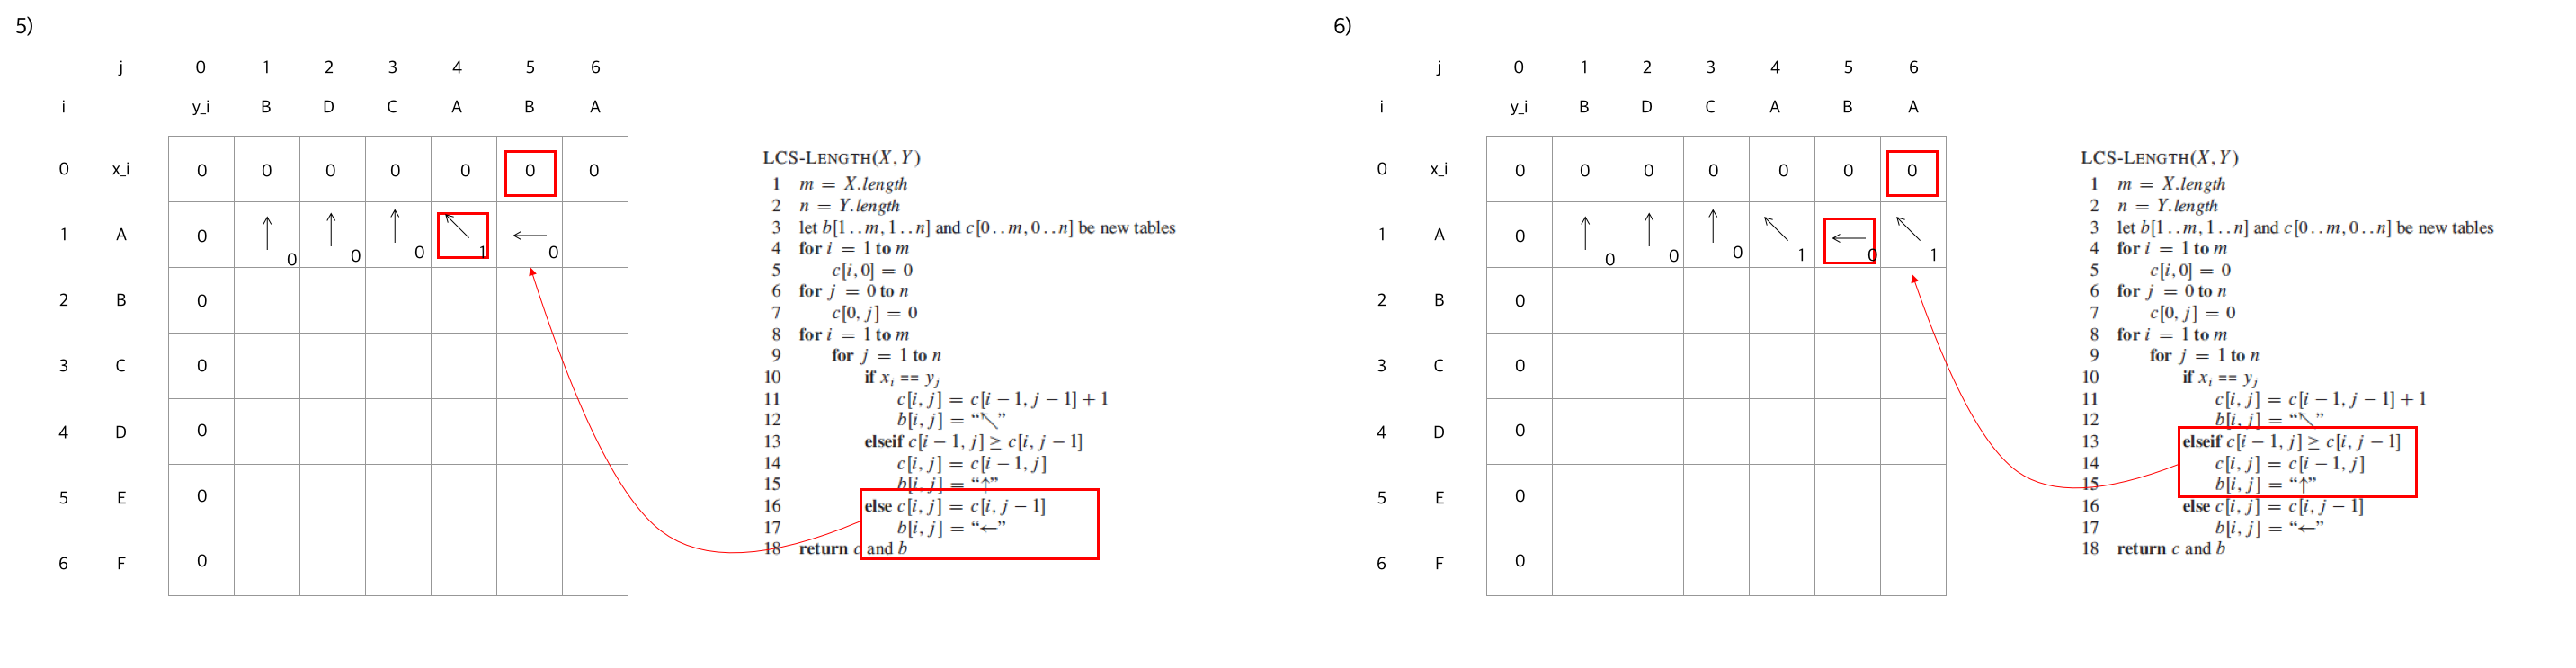
\includegraphics[width=\linewidth]{images/worksheet_3_solution_15.png}
                    \end{center}

                    \item compute $i = 2$ (needs revision)

                    \begin{center}
                    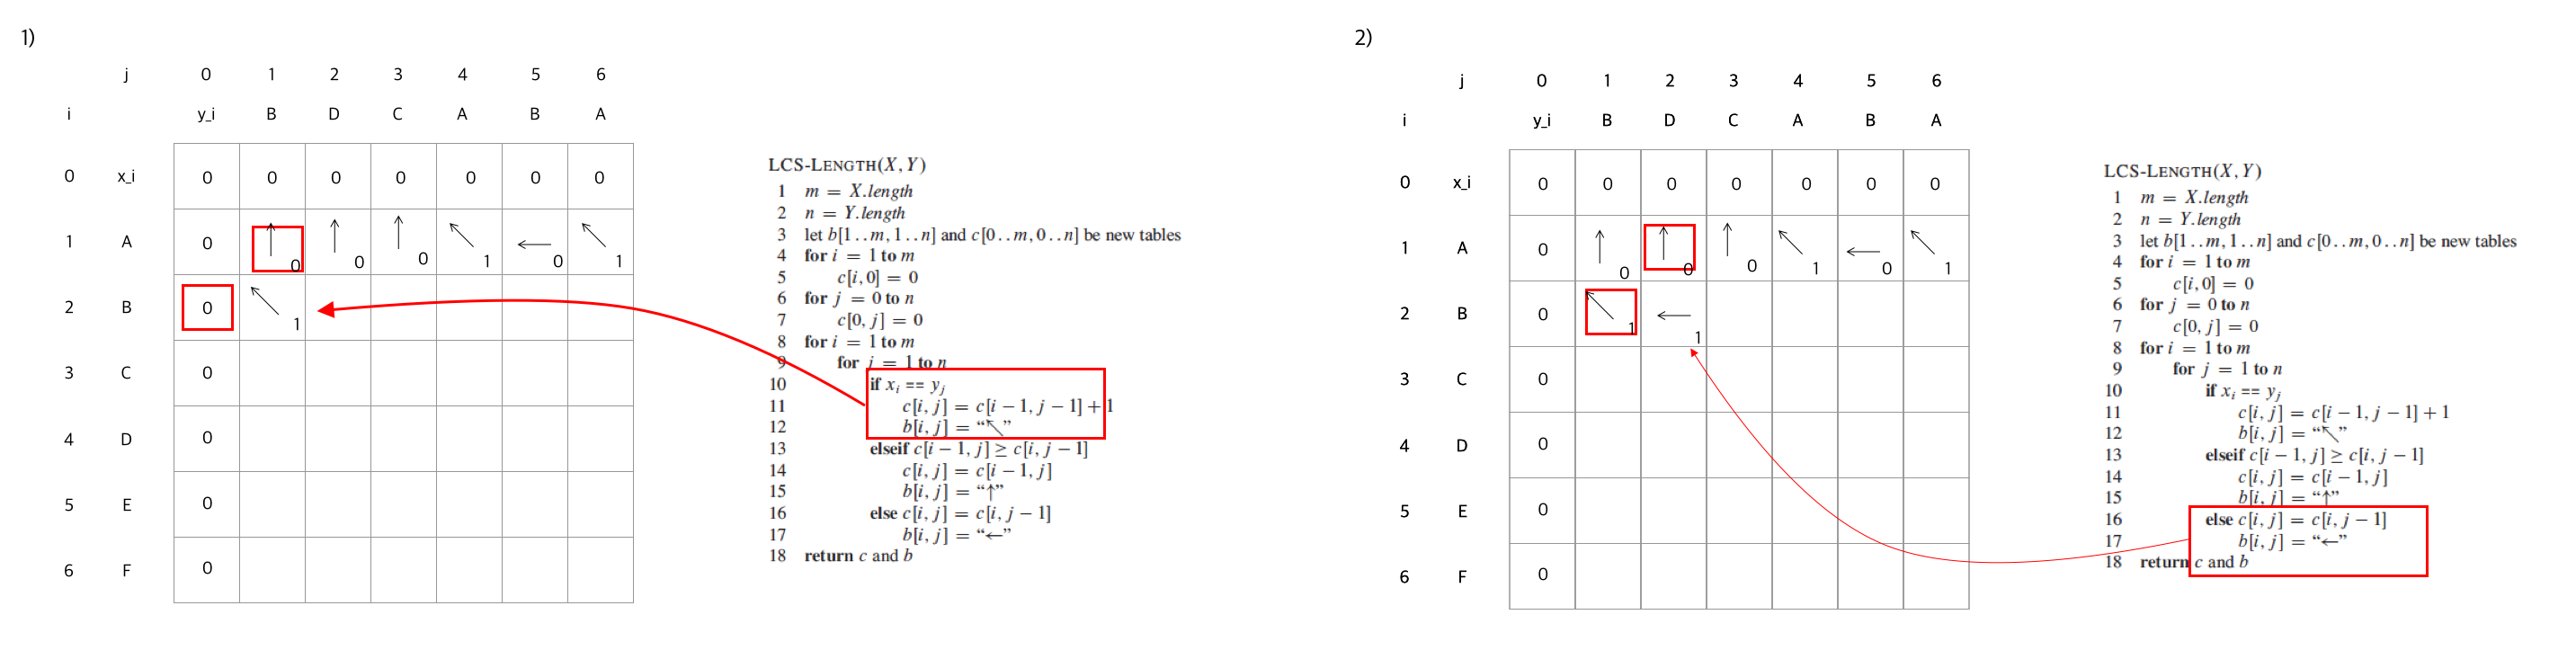
\includegraphics[width=\linewidth]{images/worksheet_3_solution_16.png}
                    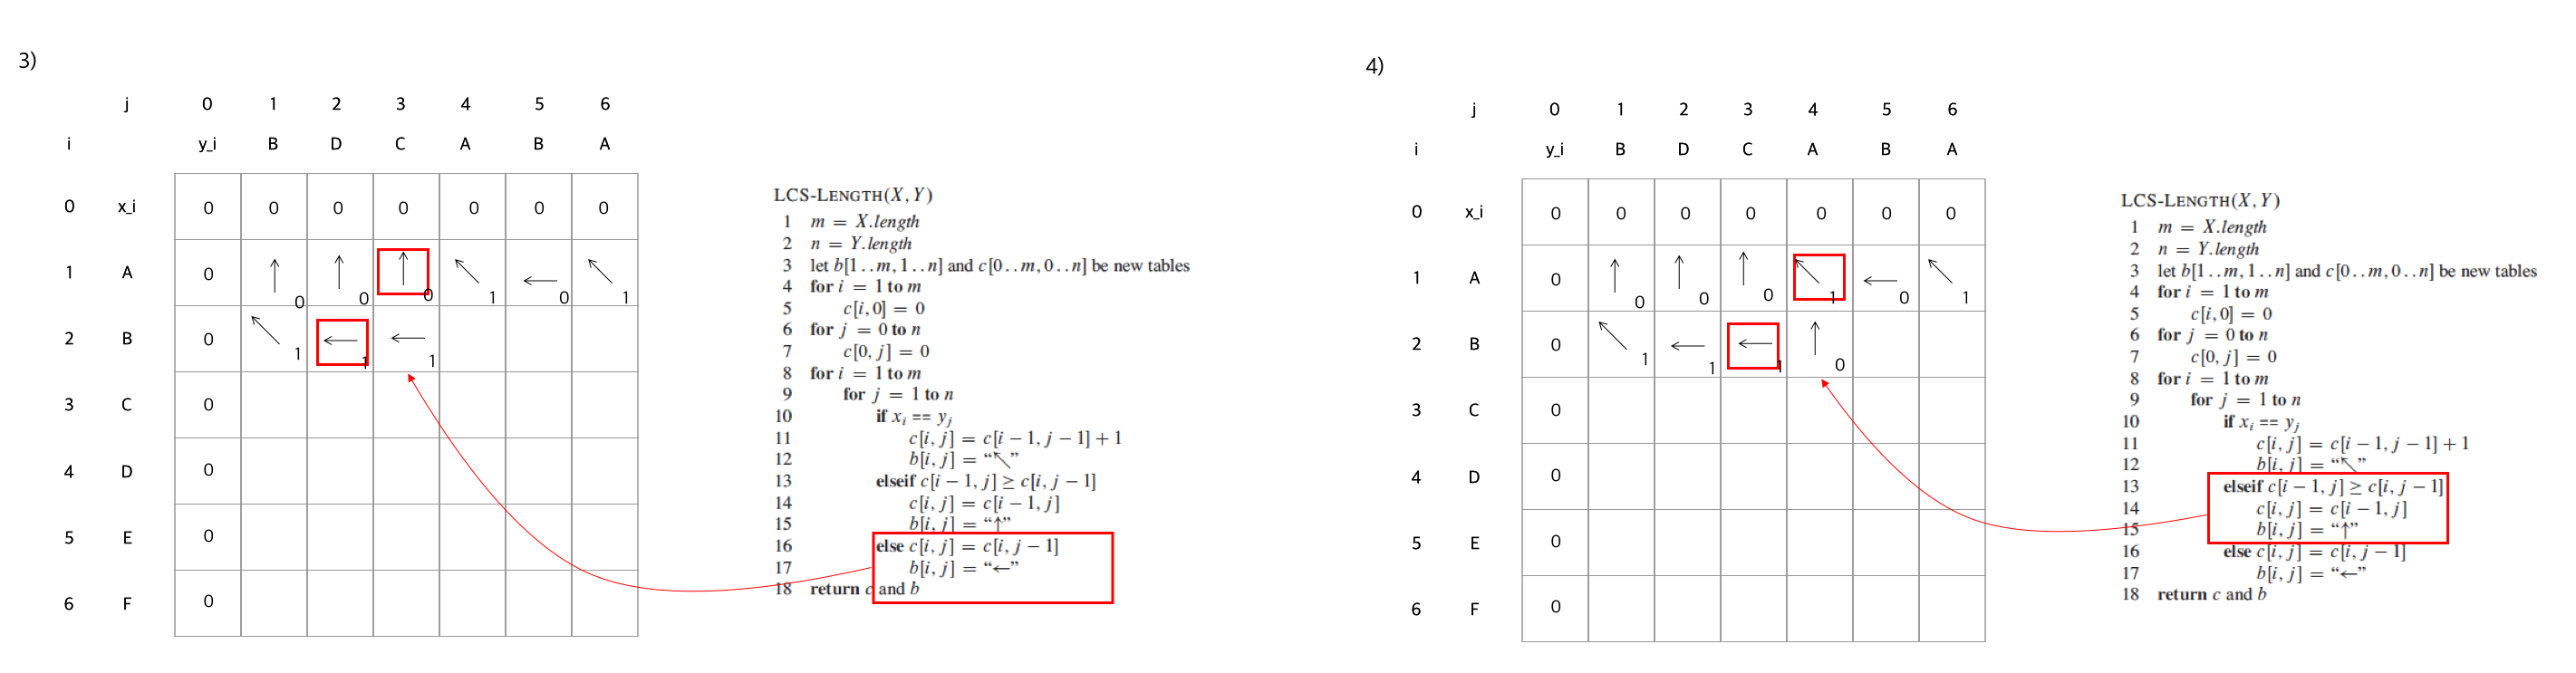
\includegraphics[width=\linewidth]{images/worksheet_3_solution_17.png}
                    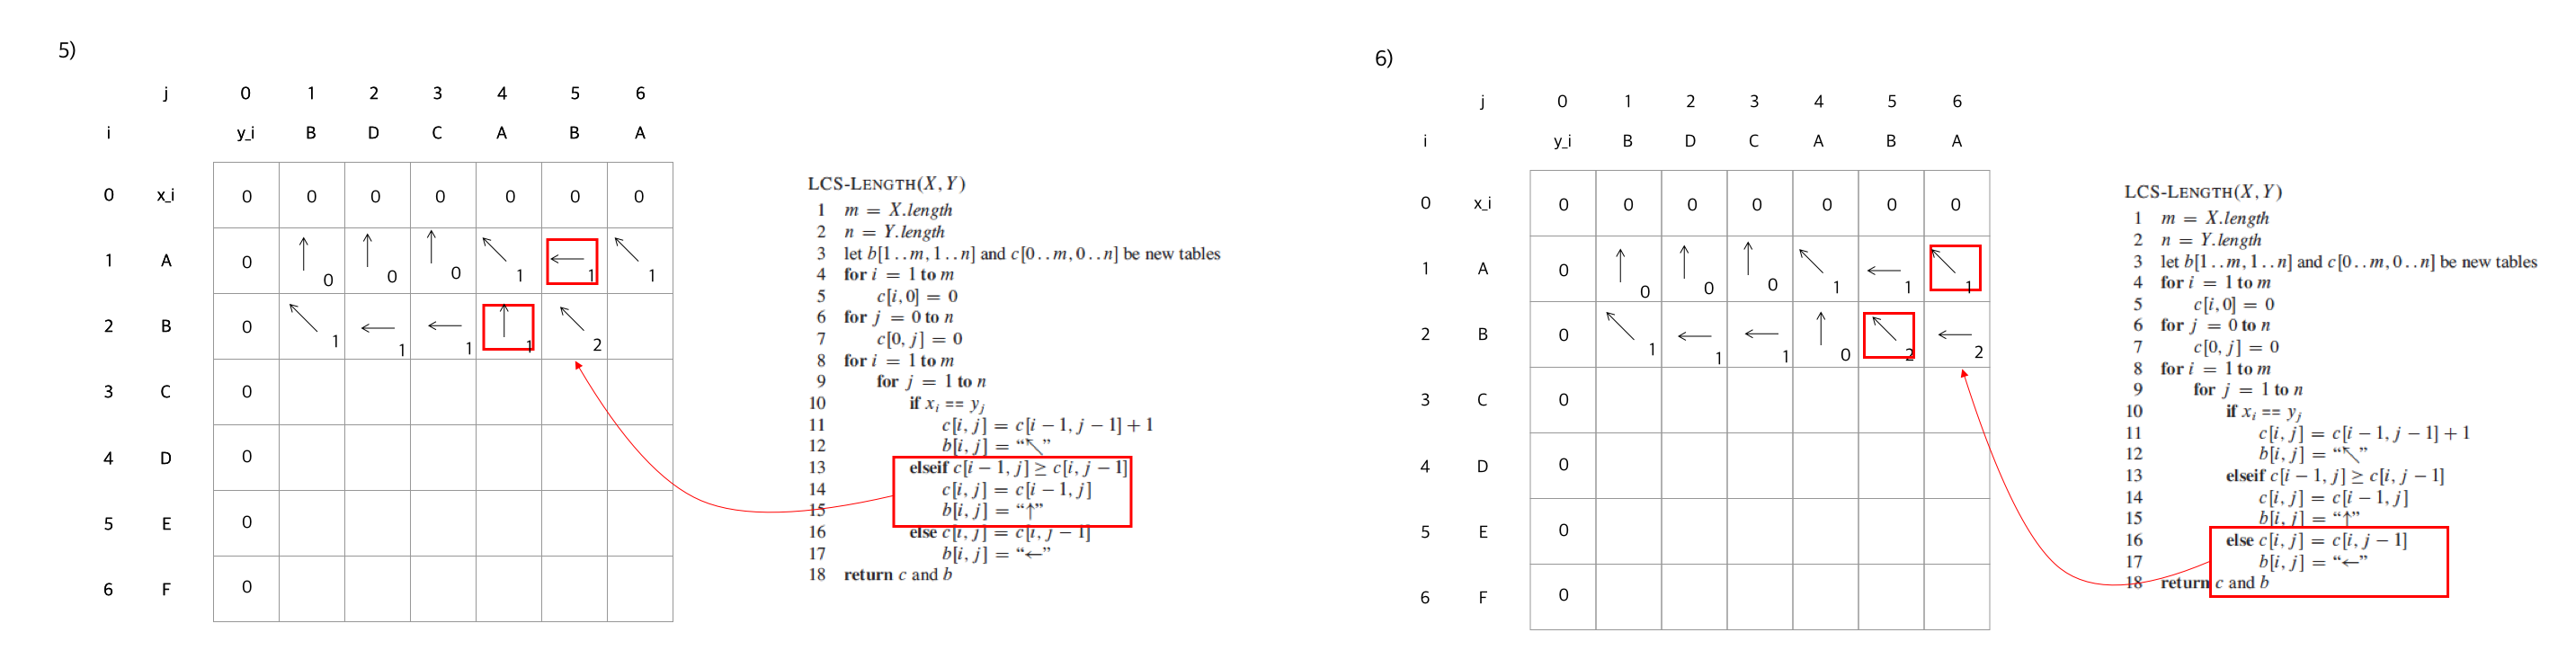
\includegraphics[width=\linewidth]{images/worksheet_3_solution_18.png}
                    \end{center}

                    \item Compute other entries using the same steps as above

                    \item Reconstruct LCS

                    \begin{itemize}
                        \item Follow the arrows   the \textbf{lower right-hand corner}
                        \item Select all `$\nwarrow$'
                    \end{itemize}

                    \bigskip

                    \begin{center}
                    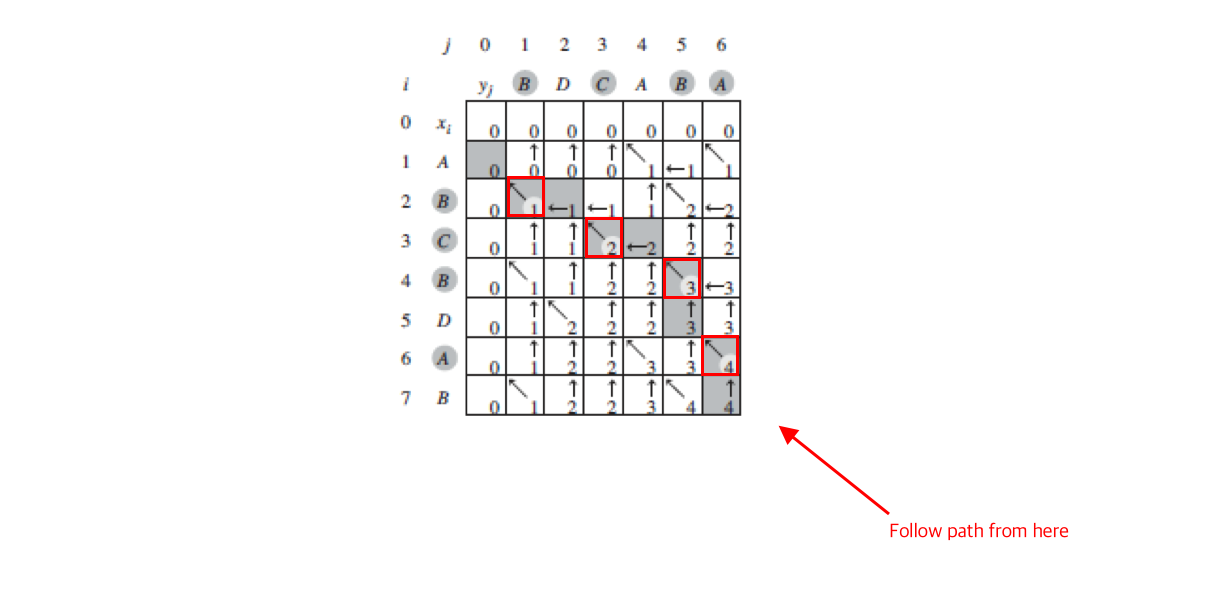
\includegraphics[width=\linewidth]{images/worksheet_3_solution_19.png}
                    \end{center}


                    \bigskip

                    Here, the result is `BCBA'


                \end{enumerate}
            \end{enumerate}
        \end{itemize}
    \end{itemize}

    \item

    \begin{lstlisting}[mathescape=true]
    PRINT-LCS(c,X,Y,i,J)
        if i == 0 or j == 0
            return
        if X[i] == Y[i]
            PRINT-LCS(c,X,Y,i-1,j-1)
            print X[i]
        elseif c[i-1, j] $\geq$ c[i, j - 1]
            PRINT-LCS(c,X,Y,i-1,j)
        else
            PRINT-LCS(c,X,Y,i,j-1)
    \end{lstlisting}

    \item

    \begin{lstlisting}[mathescape=true]
    LIS(A)

        let B be new array
        j = 0

        for i = 0 to n
            if i = 0
                B[j] = A[i]

            elseif A[i] < max(B)
                REPLACE-NEXT-VALUE-IN-B-BIGGER-THAN-Ai(B,A[i]) #Done using binary search

            elseif A[i] $\leq$ B[j]
                B[j] = A[i]
            else
                j += 1
                B[j] = A[i]

        return B
    \end{lstlisting}

    \bigskip

    \begin{mdframed}
        \underline{\textbf{Correct Solution:}}

        \bigskip

    \begin{lstlisting}[mathescape=true]
    LIS(A)

        let B be new array
        j = 0

        for i = 0 to n
            if i = 0
                B[j] = A[i]

            elseif A[i] $\leq$ B[j]
                B[j] = A[i]
            else
                j += 1
                B[j] = A[i]

        return B
    \end{lstlisting}
    \end{mdframed}

    \bigskip

    \underline{\textbf{Notes:}}

    \bigskip

    \begin{itemize}
        \item Longest Increasing Subsequence

        \begin{itemize}
            \item LIS $\to$ LCS but a minor variation

            \begin{itemize}
                \item Is the same as LCS's

                $A = <x_1, x_2, x_3, ..., x_n>$

                $B = <min(A), min(A) + 1, ... , max(A)>$
            \end{itemize}
            \item Finds the longest and largest monotonically increasing subset of numbers

            \bigskip

            \underline{\textbf{Example:}}

            \bigskip

            $2,1,7,4,6,12,9,13,15$

            \bigskip

            \begin{center}
            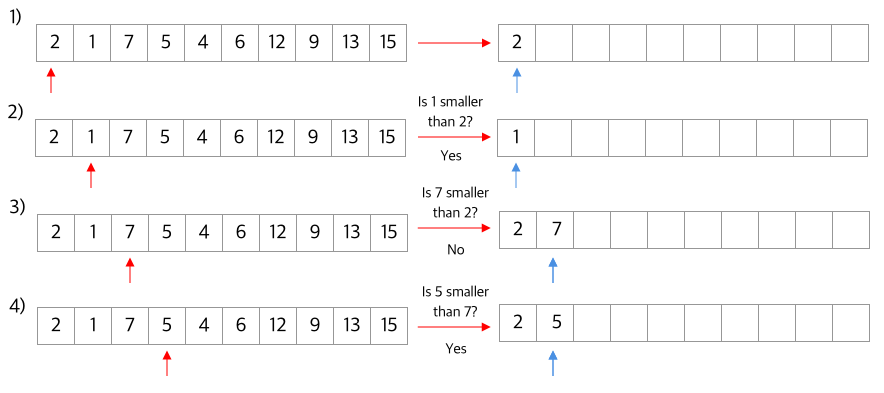
\includegraphics[width=\linewidth]{images/worksheet_3_solution_21.png}
            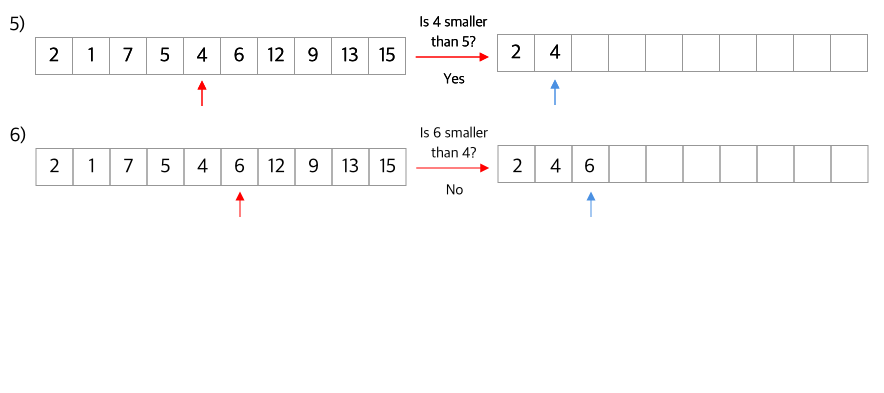
\includegraphics[width=\linewidth]{images/worksheet_3_solution_22.png}
            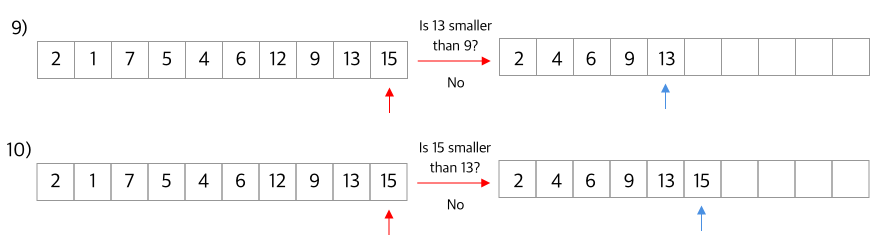
\includegraphics[width=\linewidth]{images/worksheet_3_solution_23.png}
            \end{center}

            \bigskip

            \underline{\textbf{Example 2:}}

            \bigskip

            $2,1,7,4,6,12,9,13,15,3$

            \begin{center}
            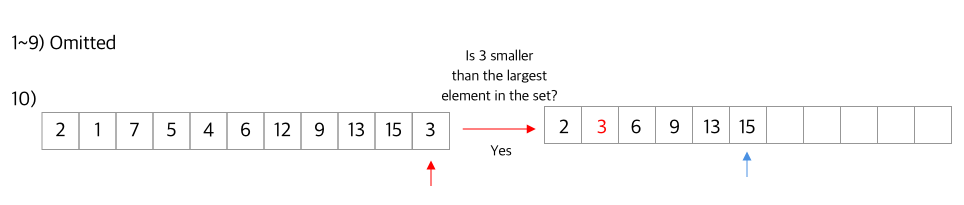
\includegraphics[width=\linewidth]{images/worksheet_3_solution_24.png}
            \end{center}

            \item Considers values and not indices

            \begin{itemize}
                \item
            \end{itemize}
        \end{itemize}
    \end{itemize}
    \item

    \bigskip

    \underline{\textbf{Rough Work:}}

    \bigskip

    \textbf{Goal:} Find the longest palindromic subsequence, and return its length

    \bigskip

    \textbf{Example:}

    \bigskip

    $<A> \to 1$

    $<A,B,A> \to 3$

    $<A,B,B> \to 2$

    $<A,A,B> \to 2$

    \bigskip

    \underline{Brute Force Method}

    \begin{itemize}
        \item For each combination of subsequence, check if substring
        is palinrome

        \begin{itemize}
            \item If palindrome,

            \bigskip

            Check if is the longest

            \bigskip

            \begin{itemize}
                \item If longest, replcae the value of a variable
                containing the current largest palindromic substring
            \end{itemize}

        \end{itemize}
    \end{itemize}

    \bigskip

    \underline{Improved Solution}

    \begin{itemize}
        \item Start at string with full length
        \item Check if palindrome

        \begin{itemize}
            \item If palindrome

            \bigskip

            Return length
            \item if not palindrome

            \begin{itemize}
                \item Return the length of largest paldromic subsequence
                by decreasing the RHS bound of the sequence to left by 1

                \bigskip

                i.e

                \bigskip

                $[A,A,B] \to [A,A],B \to \text{Return 2}$

                \item Return the length of largest paldromic subsequence
                by increasing the LHS bound of the sequence to right by 1



                \bigskip

                i.e

                \bigskip

                $[A,A,B] \to A,[A,B] \to \text{Return 1}$

                \bigskip

                \item

                If $a \geq b$, return a

                \bigskip

                else return b
            \end{itemize}
        \end{itemize}

        \bigskip

    \begin{lstlisting}[mathescape=true]
    Longest-Palindrome-Subsequence(A,i,j)
        if Palindrome(A,i,J)
            return length(A[i..j])

        a = Longest-Palindrome-Subsequence(A, i, j - 1)
        b = Longest-Palindrome-Subsequence(A, i + 1, j)

        if a $\geq b$
            return a
        else
            return b
    \end{lstlisting}

    \bigskip

    Here in this case, the algorithm has time complexity of $O(2^n)$.

    \bigskip

    \underline{Improved Solution \# 2}

    \bigskip

    \begin{itemize}
        \item Define 2D table T[i,j]

        \begin{mdframed}
        Let $T$ be 2-D table where $T[i,j]$ contains the length of longest palindromic
        subsequence $<x_i,...,x_j>$.
        \end{mdframed}

        \item Define T[i,j] when $x_i = x_j$ and $x_i \neq x_j$

        \begin{mdframed}
        Now, I need to define $T[i,j]$ when $x_i = x_j$ and $x_i \neq x_j$.

        \bigskip

        When $x_i = x_j$, we can write the length of longest palindromic subsequence $T[i,j]$
        is 2 more than $T[i+1,j-1]$.

        \bigskip

        At case $i = j$, $T[i,j] = 1$.

        \bigskip

        So, we have $T[i,j]=T[i+1,j-1] + 2$ if $i < j$ and $T[i,j] = 1$ is $i = j$.

        \bigskip

        When $i < j$ and $X[i..j]$ is a part of longest palindromic subsequence , then $T[i,j]$



        \bigskip


        \end{mdframed}

        \item Write recursive formula

        \item Write for-loops
    \end{itemize}

    \end{itemize}
    \underline{\textbf{Notes:}}

    \bigskip

    \begin{itemize}
        \item \textbf{ith Prefix} of a sequence is a subsequence of a sequence of length $i$ that occurs at the beginning of the sequence.

        \bigskip

        \underline{\textbf{Example:}}

        \bigskip

        $X = <A,B,C,B,D,A,B>$

        \bigskip

        Then

        \bigskip

        $X_4 = <A,B,C,B>$
    \end{itemize}
\end{enumerate}

\end{document}